%Made By Thomas Debelle
%Ajouté des Packages si nécessaires
\documentclass{report}
\usepackage[a4paper, total={7in, 10in}]{geometry}
\usepackage[utf8]{inputenc}
\usepackage[english]{babel}
\usepackage{graphicx}
\usepackage{graphics}
\usepackage[T1]{fontenc}
\usepackage{amsmath}
\usepackage{hyperref}
\usepackage{amssymb}
\usepackage{listings}
\usepackage{xcolor}
\usepackage{array}
\usepackage{float}
\usepackage{amsfonts}
\usepackage{fancyhdr}
\usepackage{titlesec}
\usepackage{xparse}
\usepackage{wrapfig}

\definecolor{codegreen}{rgb}{0,0.6,0}
\definecolor{codegray}{rgb}{0.5,0.5,0.5}
\definecolor{codepurple}{rgb}{0.58,0,0.82}
\definecolor{backcolour}{rgb}{0.95,0.95,0.92}

\lstdefinestyle{mystyle}{
    backgroundcolor=\color{backcolour},   
    commentstyle=\color{codegreen},
    keywordstyle=\color{magenta},
    numberstyle=\tiny\color{codegray},
    stringstyle=\color{codepurple},
    basicstyle=\ttfamily\footnotesize,
    breakatwhitespace=false,         
    breaklines=true,                 
    captionpos=b,                    
    keepspaces=true,                 
    numbers=left,                    
    numbersep=5pt,                  
    showspaces=false,                
    showstringspaces=false,
    showtabs=false,                  
    tabsize=2
}

\lstset{style=mystyle}

\hypersetup{
    colorlinks=true,
    linkcolor=black,
    filecolor=magenta,
    urlcolor=cyan,
    pdftitle={Summary DDP},
    pdfpagemode=FullScreen,
    }
\begin{document}

%Si la mention "Juin 2023" est sur une autre page, changé le dernier VSPACE
\begin{titlepage}
    \begin{figure}
        \includegraphics[height = 2cm]{KUL_Logo.png}
        \label{fig:my_label}
    \end{figure}

    \hspace*{100cm}
    \centering
    \vspace*{7cm}

    {\Huge \textbf{Summary - Design of digital platforms}}\\
    \vspace*{0.25cm}
    Version of \today\\
    \vspace*{0.25cm}
    \Large{Thomas Debelle}\\

    \vspace*{9cm} %Le dernier VSPACE
    {\Large January 2025}
\end{titlepage}

%_____NE PAS MODIFIER______
\tableofcontents
\newpage

\chapter{First Part}

\section{What is a digital platform?}

It is a collection of \textbf{digital hardware} (with embedded firmware) that can be used to bring a solution for a given class (or classes) of applications.

So typically some general purpose board like an Arduino is an example.

We have a sort of sensory swarm at the edge of the cloud that is composed of trillions of connected devices listening and sending data to each other. Often this flow of data goes back to the cloud.

\section{What matters when I design a digital platform?}

We have various constraint that limits the design of digital platform : 
\begin{itemize}
    \item Power and energy
    \item Throughput and latency (time)
    \item Cost (NRE and Area)
    \item Flexibility
\end{itemize}

\subsection{Power and Energy}

We know that $P = V \times I$ which is instantaneous. It's an important metric when designing a cooling solution.
On the other hand $Energy = P \times t$ so how long this device is on at what power rate. So we can have devices that consume a lot of power in small bursts that will ultimately use less power.

We care the most about the energy since most of the SWARM is running on battery so limited source of energy. For cloud energy is less important but having a large amount of power and so energy can quickly scale up to enormous means of electricity production.

\subsection{Throughput and latency}

\begin{itemize}
    \item \textbf{\textit{Throughput :}} It is the amount of data processed per \textit{time unit}. So we can link this to the sampling frequency. A sample can be an amount of Giga bytes or Pixels per second.
    \item \textit{\textbf{Latency :}} It is the delay between input and output. Really matters for system with feedback ! Above $100$ ms it is noticeable.
    \item \textit{\textbf{Critical Path :}} associated with the implementation which is the longest path between two clocked elements. So it defines the \textbf{max clock frequency}.
    \item \textit{\textbf{Sample frequency}}: it is not equal to the clock frequency it indicates how many time a certain process need to be done and so sampled.
\end{itemize}

Usually embedded systems have real time constraint which are HARD constraints.

\subsection{Cost}

\begin{enumerate}
    \item Recurring costs : so costs linked to the production of a chip and proportionate to the size of produced chips.
    \item Non-Recurrent Engineering cost : the pay of the engineers.
\end{enumerate}

So it is typical to have higher NRE for smaller quantities chips than Recurring costs.

\begin{figure}[H]
    \centering
    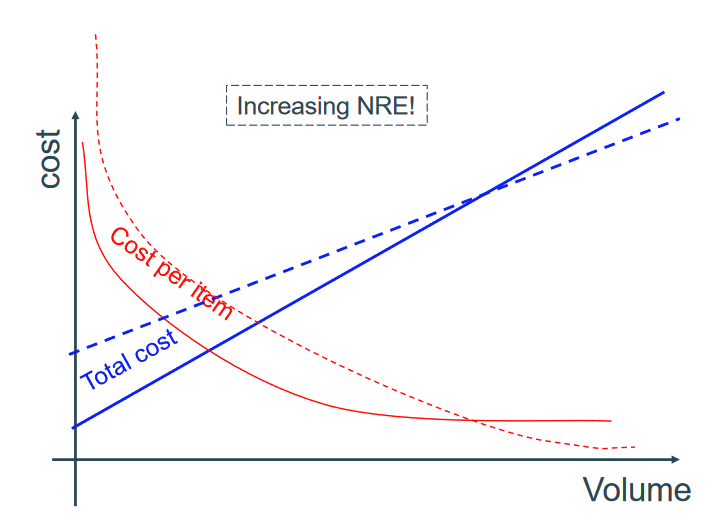
\includegraphics[width=0.5\linewidth]{typical_nre.png}
    \caption{Typical grow of costs with volume}
    \label{fig:nre-label}
\end{figure}


\subsection{Flexibility}

\begin{figure}[H]
    \centering
    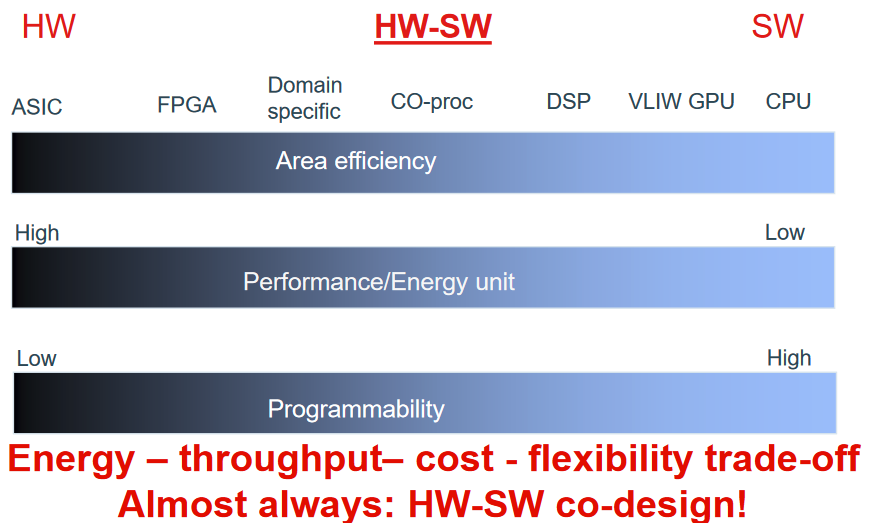
\includegraphics[width=0.75\linewidth]{flexibility.png}
    \caption{Flexibility of various platform choices}
    \label{fig:platform-label}
\end{figure}

We need to find a balance between software and hardware programming to find the best performance balance.

\begin{center}
\begin{tabular}{| m{3cm} | m{8cm}| m{1.5cm} |}
    \hline
    type & Description & HW/SW \\
    \hline
    \hline
    General Purpose Processor & 
    They are the basics CPU in computer composed of an instruction sets that is standardized. & SW \\
    \hline
    ASIC & Or Application Specific Integrated Circuit. It uses \textbf{hardwired logic} and we program it using some HDL such as Verilog to synthesize in gates and to drive to layout & HW \\
    \hline
        Reconfigurable logic & We can program on it after fabrication using FPGA (Field Programmable Gate Away). & HW-SW \\
    \hline
        ASIP & they are Application/Domain specific instruction set processor. They are often processors with new and customs instruction set (DSP, crypto, ...) and need a datapath update. & HW-SW \\
    \hline
        Mix & We can cobine the GP and SP continuum to keep flexibility and yet be efficient. Processor + FPGA & HW-SW \\
    \hline
    
\end{tabular}
\end{center}

\section{Design methodology of a digital platform?}

\begin{itemize}
    \item Methodology is a set of \textbf{practices} that, when applied in the right sequence, allow engineers to design the right system correctly within a given cost and time budget
    \item Design flow is a systematic \textbf{sequence} of well defined design activities that, in a time and cost effective way, leads to a production plan
\end{itemize}

It's a top to bottom approach where we first design in software and then in hardware.

\subsection{Y-Chart (Gajski-Kuhn)}

\begin{figure}[H]
    \centering
    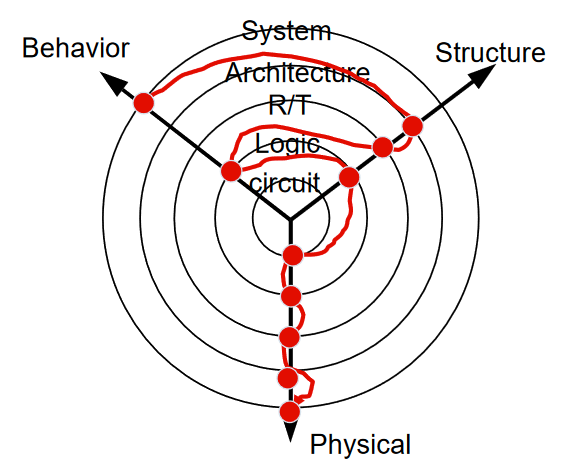
\includegraphics[width=0.5\linewidth]{Y-chart.png}
    \caption{Y-chart}
    \label{fig:y-chart-label}
\end{figure}

So we alternate between behavior and structure to finally implement the physical. We do some \textbf{horizontal exploration} at each layer to be able to better implement. To do "what" (IO behavior) $\rightarrow$ "how" (composition) $\rightarrow$ "implement" (realization). 

\begin{center}
\begin{tabular}{| m{3cm} | m{8cm}| m{4cm} |}
    \hline
    Layer & Description & tools\\
    \hline
    \hline 
    1. System Level & We start with informal specs, use of abstract Data types. Check if we are doing the right system & Python, C, Matlab, ... \\
    \hline 
    2. Architecture Level & Optimize the process (algorithm), Architectural Mapping (HW/SW), chip floorplan (chip building). Stage where we are making the biggest gain (70\%) & mix of HW and SW \\
    \hline 
    3. Register Transfer Level & We create some Finite State Machine with Datapath and introduce time and signal. & Synchronous design with FSM and DP actions. \\
    \hline 
    4. Logic Level Design for ASIC back-end &  We now use boolean expressions, FSM, ... We introduce \textit{delay} & FSM, Clocked VHDL, bits, Gates, ... \\
    \hline 
    5. Circuit Level & Transistor schematic, layout strategy, logic cell layout, transistor dimension, voltages, ... & Transistors \\
    \hline
    
\end{tabular}
\end{center}

When going through those steps there is a lot of back and forth to find the right implementation since it is a non trivial problem.

\subsubsection{Design activites at Register Transfer}

To increase sampling frequency we can do some \textbf{time multiplexing} which will help to execute something let's say in one clock cycle by doubling the hardware compared to a 1 hardware 2 clock cyle. To do the \textbf{3.} level we need to clearly indicate all \textbf{flip-flop} with a $>$ and all the IO size of wires. It is also a good thing to highlight the critical path in a design.

We have 3 main tasks here that are :
\begin{enumerate}
    \item \textit{\textbf{Scheduling :}} Decide the clock cycle for each \textbf{operation}. We can either look for minimum execution time, minimum hardware.
    \item \textit{\textbf{Allocating :}} How many \textbf{operators} of each time are required (addition, multiplication, ...)
    \item \textit{\textbf{Assigning :}} Deciding which \textbf{operations} goes with each \textbf{operators}. We also need to assess the issue and possible design problem with our choices.
\end{enumerate}

We will often usee Data Flow Graph representation (more on that at \ref{DFG}). We also need to take into account the reality of hardware at this step.

\subsubsection{Logic Design Activities}

We use again some logic and FSM synthesis. We are now going to map this on a chip with cells having an actual purpose and limited operations. We look for the critical logic path and delay issues. P\& R C extraction from wiring.

We will first validate the design by checking syntax, connections, for synthesizable components ! We may get some warning or errors. Then it will generate us a \textit{net-list} which is similar to a binary executable and can converts logic expressions into gate level expressions. So we have now an idea about the area and the time.

Then the map will synthesize net-list into FPGA specific components (LUTS, Flip Flops) which will then generate a map net list containing all FPGA-specific components used here. Better area result but no timing.

The last step will find optimized interconnections of logic blocks. It will optimize the critical path and analyze timing constraints. It will generate a net-list with optimized logic and routing and provide final area and timing results.

\subsection{Design Methodology}

We want to avoid design iterations to cut time and cost. We need to balance the time-to-market. For that we can do : 
\begin{enumerate}
    \item Spend most of the time at the top and document. Right design right at the start
    \item Use interactive CAD tools with exploration capabilities.
    \item Keep It Simple Stupid : 
    \begin{itemize}
        \item Split function and interface. Communication needs to be simple and local
        \item Use encapsulation or wrappers
        \item reuse and plug-and-play
        \item Standardize interface
        \item Use structured interconnect
        \item Locally synchronous, Globally asynchronous
        \item Localize heavy computation and traffic
    \end{itemize}
\end{enumerate}

\section{Data Flow Model} \label{DFG}

The main issue when designing in C, it is the fact that C is sequential ! So it doesn't really simulate well how hardware works. To better represent concurrent execution we will prioritize \textbf{block diagrams} and \textbf{data flow models}.

If we get the specification in C we can derive the \textit{control flow graph} or the \textit{data flow graph} from it.

\begin{figure}[H]
    \centering
    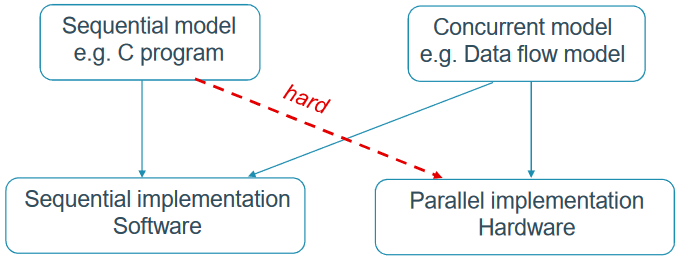
\includegraphics[width=0.5\linewidth]{specs.png}
    \caption{The difficulty of hardware implementation}
    \label{fig:hardware-impl-label}
\end{figure}

Moreover, sometimes C will consume more cycle than actually necessary and the way to accelerate the code may be obfuscated by the C code. To do so we have 2 concepts we can use :
\begin{itemize}
    \item \textit{\textbf{Concurrency :}} ability to execute \textit{simultaneous} operations because they are \textit{independent from each other}. \textbf{Property of the application}
    \item \textit{\textbf{Parallelism :}} ability to execute \textit{simultaneous} operations because we can run them \textit{on different circuit elements}. \textbf{Property of the implementation}
\end{itemize}

\subsection{Data Flow modeling}

Thanks to the DF we can show and expose \textbf{max concurrency}. It is \textbf{concurrent}, \textbf{distributed}, \textbf{modular} and \textbf{easy to analyze}.

\begin{center}
\begin{tabular}{| m{2cm} | m{5cm}|}
    \hline
    Terminology & Meaning \\
    \hline
     \hline
     Actor & Operation\\
     \hline
     Token & Carries information \\
     \hline
     Queues & Transport tokens from one actor to another\\
     \hline
     Fire & execution\\
     \hline
\end{tabular}
\end{center}

In the basic DF, we don't have any notion of time. We are using directed graph and each nodes represents a computation and each edges are a path over which the tokens travel. We just see what computations to perform not the order or sequence of them.

Later we will see \textbf{control edge} that has a relation between two operations to force a certain order of execution while a \textbf{data edge} is just a consumer and producer with data flowing on it.

\begin{figure}[H]
    \centering
    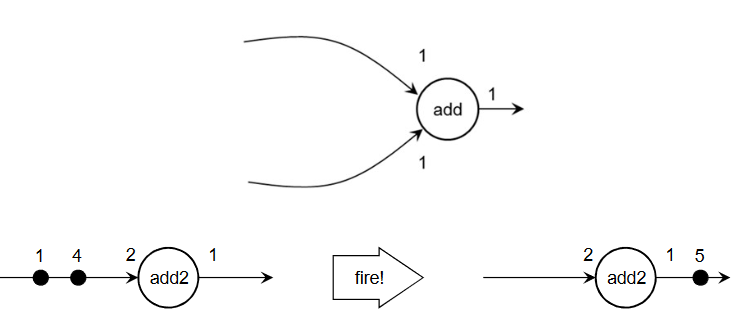
\includegraphics[width=0.5\linewidth]{ruleandrate.png}
    \caption{Firing rule, firing rate}
    \label{fig:FR-FR-label}
\end{figure}

The firing rule shows what are the conditions that needs to be met to execute the operation and the rate how much is consumed and produced.

\subsection{Synchronous Data Flow}

The number of tokens produced and consumed is known beforehand. We can then plan the amount and the firing order. We have relative sample rates and that doesn't depend on the data.

\begin{figure}[H]
    \centering
    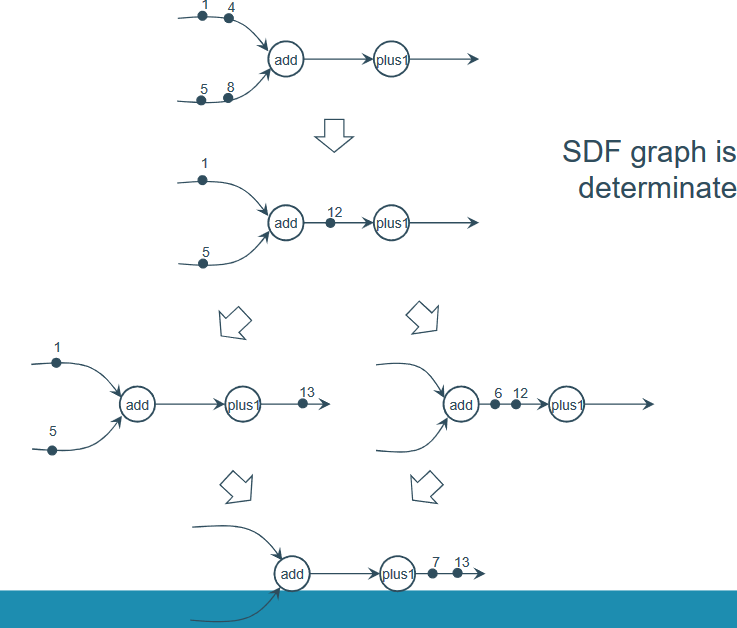
\includegraphics[width=0.5\linewidth]{sdf.png}
    \caption{SDF is determinate}
    \label{fig:SDF-label}
\end{figure}

When analyzing a SDF we can run into an admissible schedule (so no deadlock and overflowing) or non admissible schedule. We also need \textit{consistent solution} that will not lead to a deadlock and will be periodic.
To do periodic schedule for SDF we need to assume infinite stream of input data so an unbound execution. It needs to be \textbf{Periodic Admissible Sequential Schedule} (unbound execution with bounded memory).

\subsubsection{PASS Formal Approach}

We first need to construct a \textbf{topology matrix} where each column is a node and each arc is a row. We can see the production and consumption at each value.

\begin{figure}[H]
    \centering
    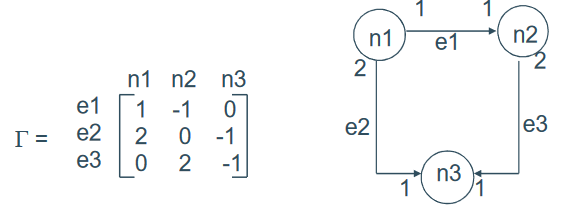
\includegraphics[width=0.5\linewidth]{topology.png}
    \caption{Topology Matrix}
    \label{fig:top-mat-label}
\end{figure}

We then have a vector $b$ indicating the size of the queues on each arc and $v$ indicating which nodes fire at a specific point in time : 

\begin{equation}
    b(n+1) = b(n) + \Gamma v(n)
\end{equation}

A necessary condition is that $\Gamma$ needs to have a rank that is equal to the amount of nodes $-1$.

\subsubsection{Modeling control flow aspects}

We want to add the control-related aspects and we can by simulating control flow on top of it which will create an overhead. We can add the boolean data flow. It will make it harder to properly analyze the SDF.

\subsubsection{Adding time \& delay}

\begin{figure}[H]
    \centering
    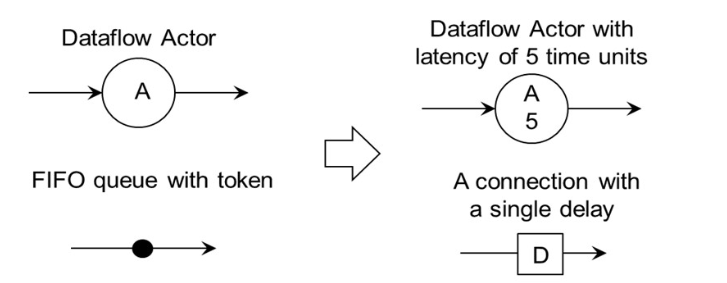
\includegraphics[width=0.5\linewidth]{sdf_time_delay.png}
    \caption{SDF with time and delay}
    \label{fig:enter-label}
\end{figure}

We now have the possibility to do some feedback and control loop. We can also add some delay on the arc.

The PASS methodology creates a topology matrix G of the SDF and verify its rank. It will determine a firing vector and try firing at each node (round robin style) until it reaches the firing vector. A good tool for this is \textbf{Ptolemy}.

\subsection{From Data flow to HW implementation}

We can first try to do some 1-to-1 mapping from dataflow to HW implementation. This will only work if we are doing some single-rate dataflow graph (so firing every 1s) and if actors are implemented in combinatorial logic. Important to use CAD tools that will find for us better structure.

For software it's way easier many implementation possible. For hardware we need to be on the look out for some possible pipelining.

\section{Transformations}

\begin{itemize}
    \item \textbf{Data Edge :} is a relation between two operations such that data produced by one operation is consumed by another.
    \item \textbf{Control Edge :} is a relation between two operations such that one operation has to be executed after the other.  
\end{itemize}

So changing a data edge will result into a different algorithm while changing a control edge will just result into another hardware realization.

We work with unit delay so each operation have unit delay and all of the queues are FIFO we need some delay for Data Flow Graph (just a block diagram) with feedback. We have the \underline{Synchronous} Data Flow Graph where we can analyze them at \textbf{design time}.

\subsection{Iteration bound}

We want to see how long it would take for one pass, amount of production etc and the storage needed for.

\begin{figure}[H]
    \centering
    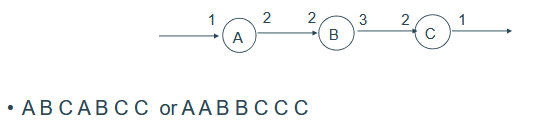
\includegraphics[width=0.5\linewidth]{pass_pass.png}
    \caption{Pass1 or Pass2}
    \label{fig:enter-pass}
\end{figure}

We will go deeper with the concept of time. First we assume an ideal queue with unit delay for every actors and operations. Then we can go to the \textit{data dependency graph} where actors have relative delays now. Later we will see the actual Hardware behind it and issues with synchronization.

The iteration period is \textit{the time required for the execution of one iteration of the algorithm}. It also indicates the max sample frequency (since we can't produce any faster).

We call a loop a path that starts and ends at the same node in a directed graph. The formula for \textbf{loop bound} is $T/W$ where T is the loop computation time and $W$  the amount of delay (since a delay could help us feeding more sample and not waiting a full loop time).

The iteration bound is the loop with the maximum loop bound and if it has no delay we have an infinity time loop (not executable).

By moving registers (delays) around we can keep the same iteration bound but lowering the critical path, the critical path can't be smaller than the iteration bound.

\subsection{Pipelining and parallelism}

\begin{itemize}
    \item \textbf{Pipelining :} reduce effective critical path by introducing pipelining latches along critical path.
    \item \textbf{Parallelism :} increases the sampling rate by replicating hardware so the several inputs can be processed in parallel and several outputs can be produced at the same time.
\end{itemize}

To add those registers we need to find \textbf{cuts} in the DFG where all the arrows point in the same directions and we can introduce some registers. It will increase the latency and the number of registers but will provide a lower critical path. This will have an impact on the power : 

\begin{equation}
    P = \alpha f C V_{DD}^2
\end{equation}

\subsection{Retiming}

The goal is to move some of the delays to change the critical path but keeping the latency as is. We use the \textbf{cutset retiming} technique which we make a cut in the DFG, add delay in one direction and remove the same amount in the other one. 

\begin{figure}[H]
    \centering
    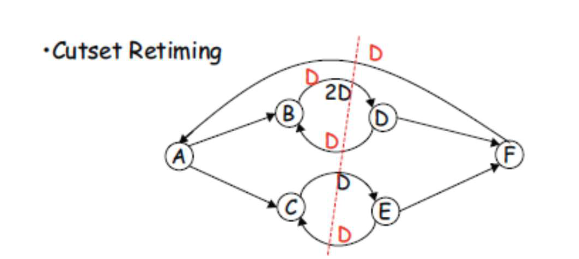
\includegraphics[width=0.5\linewidth]{cutset_retiming.png}
    \caption{Cutset Retiming}
    \label{fig:cutset}
\end{figure}

Retiming is a generalization of pipelining. General pipelining is equivalent to introducing delays at the input followed by retiming.

\subsection{Folding and unfolding}

The idea is to move from a sequential implementation towards a HW implementation that will make sure that the maximum amount of hardware is used. It's just like parallel processing.

\begin{figure}[H]
    \centering
    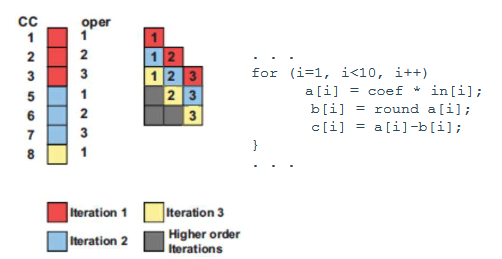
\includegraphics[width=0.5\linewidth]{Unfolding.png}
    \caption{Unfolding}
    \label{fig:unfolding}
\end{figure}

We need a program with more than 1 iteration and by applying this technique we get closer to the loop iteration bound.

\subsection{Speed-up and slow-down}

We will always have a larger clock frequency than sample frequency in most cases. Our goal is to maximize the usage. It's always a trade off between area and sample frequency, ...

\begin{figure}[H]
    \centering
    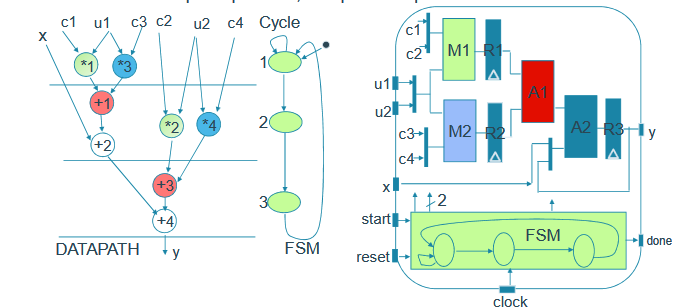
\includegraphics[width=0.5\linewidth]{example_Parallel.png}
    \caption{Example of the trade-off}
    \label{fig:parallel-label}
\end{figure}

We will reuse the same hardware but will take 3 clock cycle to produce something.

\section{From C to Control Flow and Data Flow}

In this part we will try to transform algorithm to speed up the processes and find independent data, it's like using associativity, distributivity, ... and other properties to speed up everything.
\begin{lstlisting}[language=C, caption=Code Example]
int max(int a, b){
    int r;
    if (a>b){
        r = a;
    }else{
        r = b;
    }
    return r;
}
\end{lstlisting}

We first need to find all the nodes which are all the operations (function entry, variable assignation, flag creation, loops, ...). Control edges indicate all the operations and shows the order of execution. They can stay or change depending on the implementation. The data edges shows all the creation or consumption of data and the data dependencies. It shows the \textbf{flow of information} and if we change them it will fundamentally alter the algorithm.

\begin{figure}[H]
    \centering
    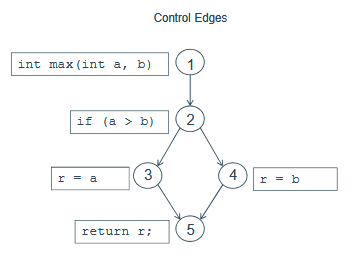
\includegraphics[width=0.45\linewidth]{control.png}
    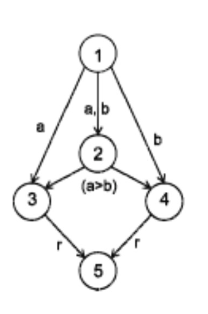
\includegraphics[width=0.2\linewidth]{data.png}
    \caption{Control and Data Edges}
    \label{fig:control-data-label}
\end{figure}

\begin{figure}[H]
    \centering
    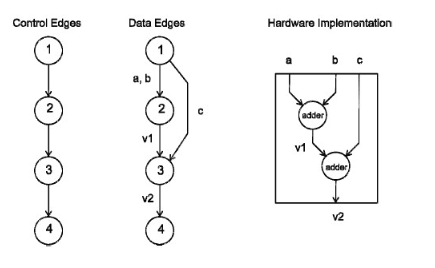
\includegraphics[width=0.5\linewidth]{dataControl2HW.png}
    \caption{Control \& Data edges to Hardware}
    \label{fig:enter-label}
\end{figure}

\subsection{Systematic Derivation of Control Flow Graph}

We know that each nodes represent a single operation and their order the order of execution.

\begin{figure}[H]
    \centering
    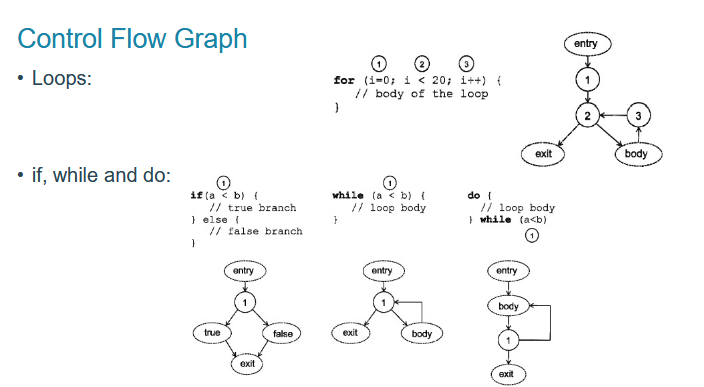
\includegraphics[width=0.75\linewidth]{Loops_cfg.png}
    \caption{Loops in CFG}
    \label{fig:loop-cfg-label}
\end{figure}

\subsection{Systematic Derivation of Data Flow Graph}

It is a bit harder to do so but we need to keep in mind that they all showcases the production and consumption of data. Each node represents one single operation. We have the same nodes as a CFG but not the same edges ! The edges always start from a read node to a production node. In conditions, we produce a flag watch out !

\subsubsection{Pointers and Arrays ?}

We need to consider each elements as a distinctive variable according to their indices. But harder for complex indices and values unknown at compile time. So we will merge all indexed variables in \textit{one single read or write}. Works well when loops are bounded at compile time.

\begin{figure}[H]
    \centering
    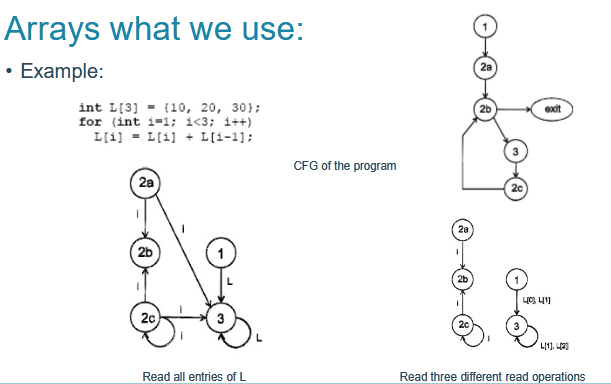
\includegraphics[width=0.75\linewidth]{complexArrays.png}
    \caption{Arrays and indices}
    \label{fig:array-index-label}
\end{figure}

\subsection{Single-Assignment Programs}

It makes the data dependency more clear and makes the life of a Hardware designer much more easy. We only assign once each variable. There is some algorithm that can do that for us.

\begin{figure}[H]
    \centering
    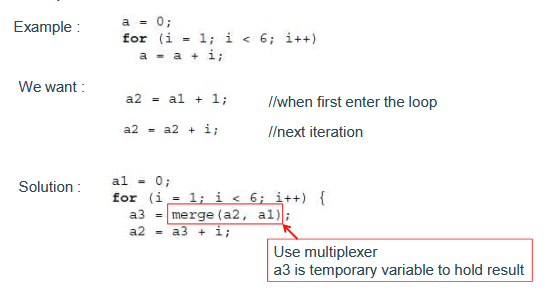
\includegraphics[width=0.75\linewidth]{SAP_loops.png}
    \caption{Single Assignment}
    \label{fig:enter-label}
\end{figure}

\begin{lstlisting}[language=C, caption=Sequential only one storage location]
int FOO(int c[4], u[4], x){
    unsigned i;
    sum = x;
    for (i=1, i<5, i++)
        sum = sum + c[i]*u[i];
    y = sum;
}
\end{lstlisting}

\begin{lstlisting}[language=C, caption=Modified single assignment]
int FOO(int c[4], u[4], x){
    unsigned i;
    sum[0] = x;
    for (i=1, i<5, i++)
        sum[i] = sum[i-1] + c[i]*u[i];
    y = sum[4];
}
\end{lstlisting}

\begin{figure}[H]
    \centering
    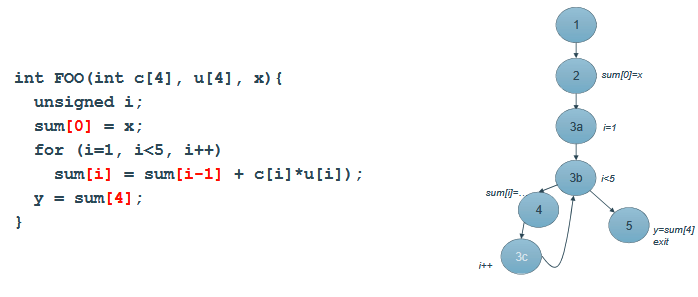
\includegraphics[width=0.75\linewidth]{CFG_single_assignment.png}
    \caption{CFG Single Assignment}
    \label{fig:enter-label}
\end{figure}

\begin{figure}[H]
    \centering
    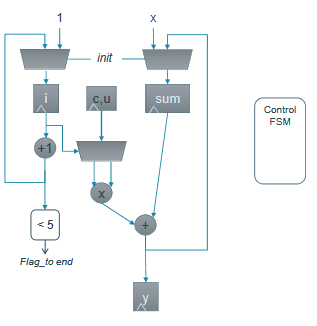
\includegraphics[width=0.5\linewidth]{Complete_HW.png}
    \caption{Complete Hardware}
    \label{fig:HW-label}
\end{figure}

We can always find ways to optimize and parallelize code ! We need to measure how many \textbf{operators} there is in our hardware and how many \textbf{operations} are in \texttt{FOO}. What is the sample frequency and the clock frequency. In this example we got :

\begin{itemize}
    \item Area : 1 mul + 1 add + 11 reg + 4 mux
    \item CP (Critical Path) : 1 mul + 1 add + 2 mux
    \item Clock freq : 4 * sample freq (derived from the delay)
    \item Latency : 4 cycles
    \item Throughput : 1/(4*CP)
\end{itemize}

The biggest optimization between software and hardware is the fact that in \textit{software} everything is \textit{sequential} and so by doing some \textit{loop unrolling, independent operations, ...} we can optimize all of this. The key is to \textbf{bring as much parallelism as possible} by unrolling everything. From there we can Redraw the CFG and DFG :

\begin{figure}[H]
    \centering
    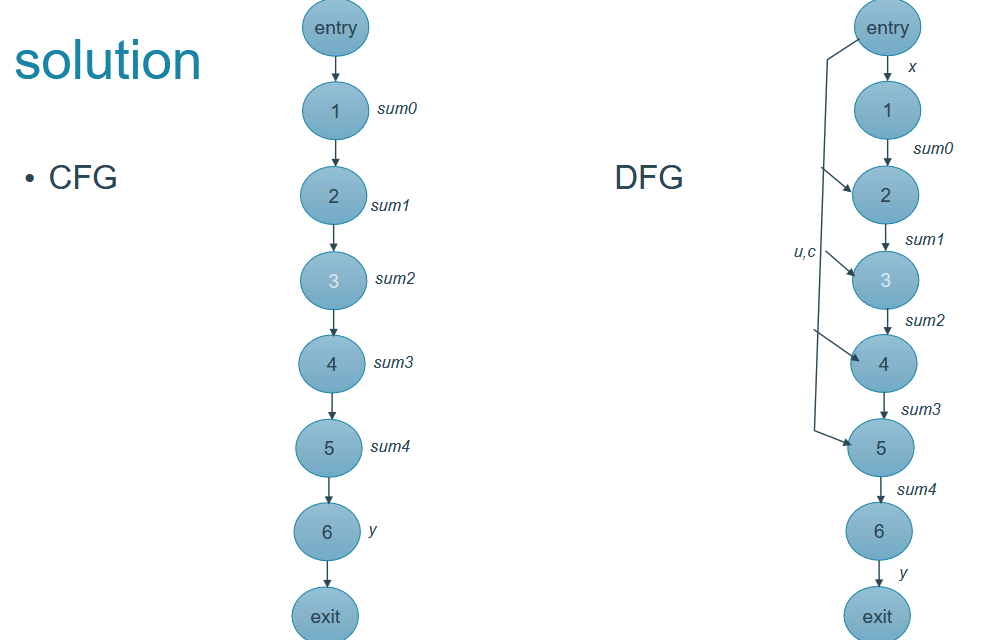
\includegraphics[width=0.75\linewidth]{img/unroll.png}
    \caption{After unrolling}
    \label{fig:enter-label}
\end{figure}

After this DFG, we can redraw the HW implementation but we can also decide to run in parallel because as it is, we will use a lot of adder but we want to maximize their utilization : 

\begin{itemize}
    \item Area : 4 mul + 4 add + 10 reg
    \item CP : 1 mul + 3 add + 1 reg
    \item Clock freq : sample freq (derived from the delay)
    \item Latency : cycle
    \item Throughput : 1/(CP)
\end{itemize}

\begin{figure}[H]
    \centering
    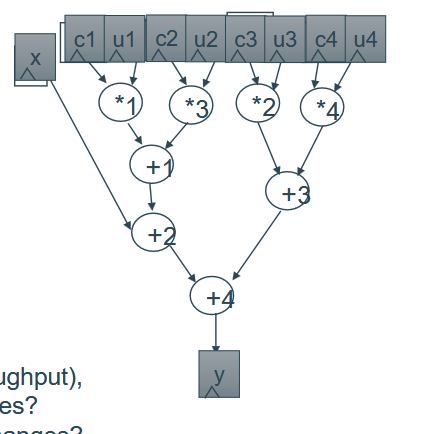
\includegraphics[width=0.5\linewidth]{img/optimize_HW.png}
    \label{fig:enter-label}
\end{figure}

So to speed-up things we can use \textbf{pipeline} and \textbf{parallelize}. To slow down things we can use \textbf{time multiplexing} and reuse some hardware etc to reduce the area.

\begin{figure}[H]
    \centering
    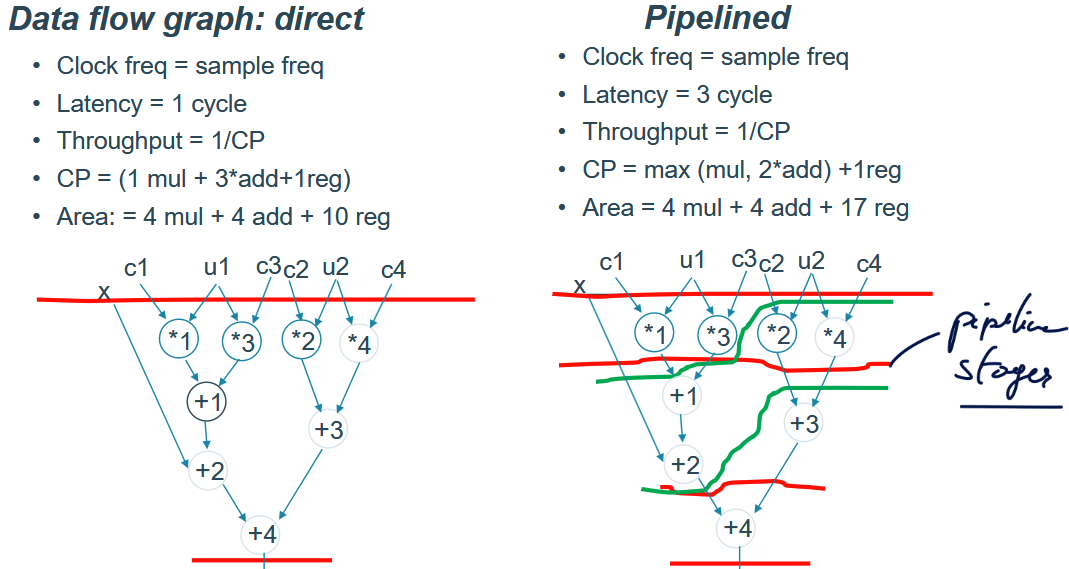
\includegraphics[width=0.45\linewidth]{img/pipeline.png}
    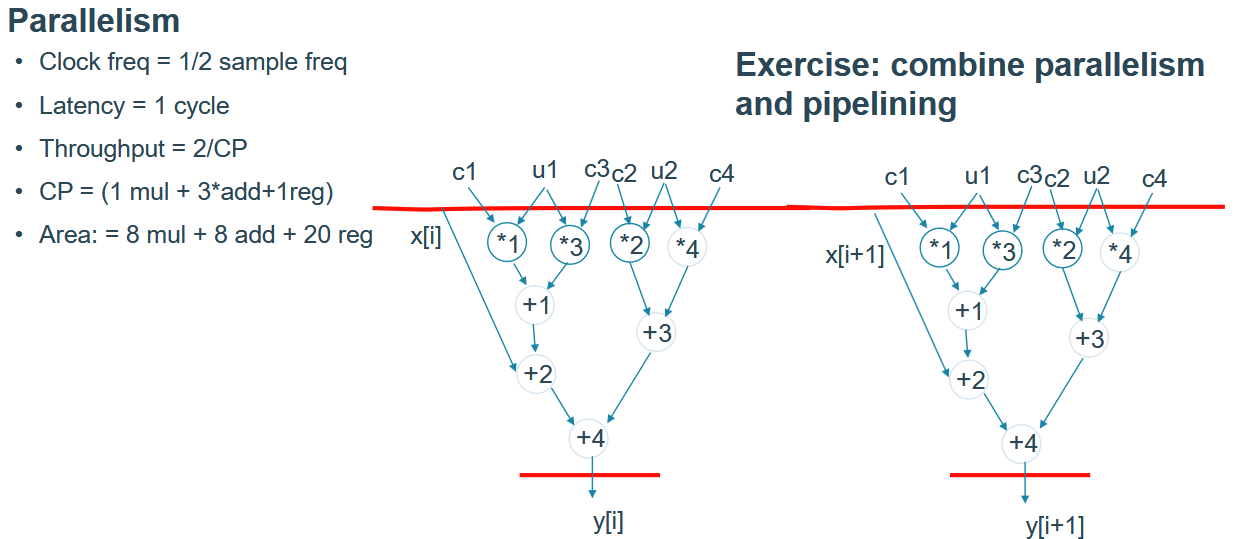
\includegraphics[width=0.54\linewidth]{img/parallelism_example.png}
    \caption{Pipeline induce less timing constraints so higher Clock Frequency, Parallelism more TP}
    \label{fig:enter-label}
\end{figure}

\begin{figure}[H]
    \centering
    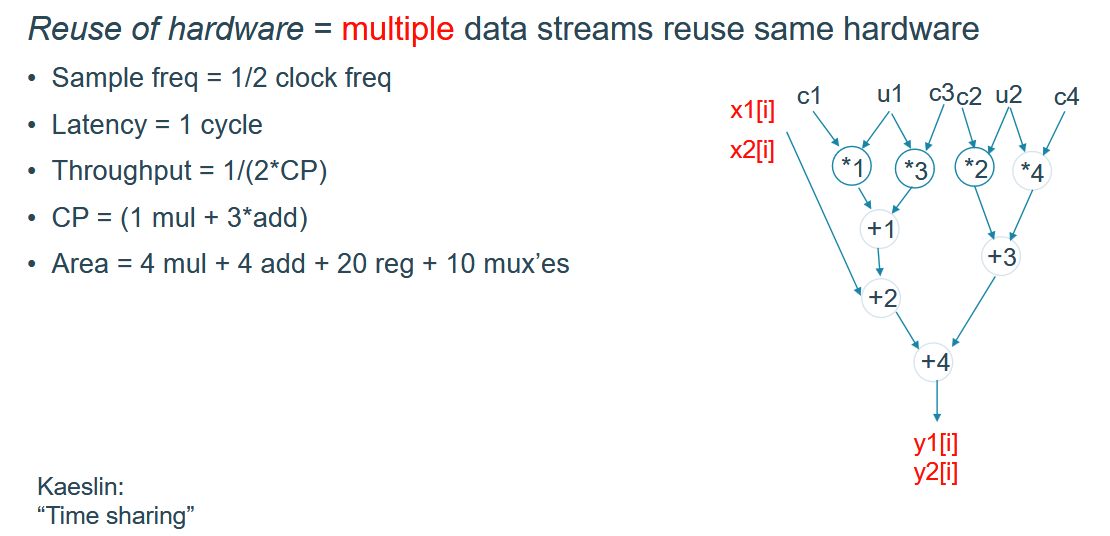
\includegraphics[width=0.45\linewidth]{img/slow_down.png}
    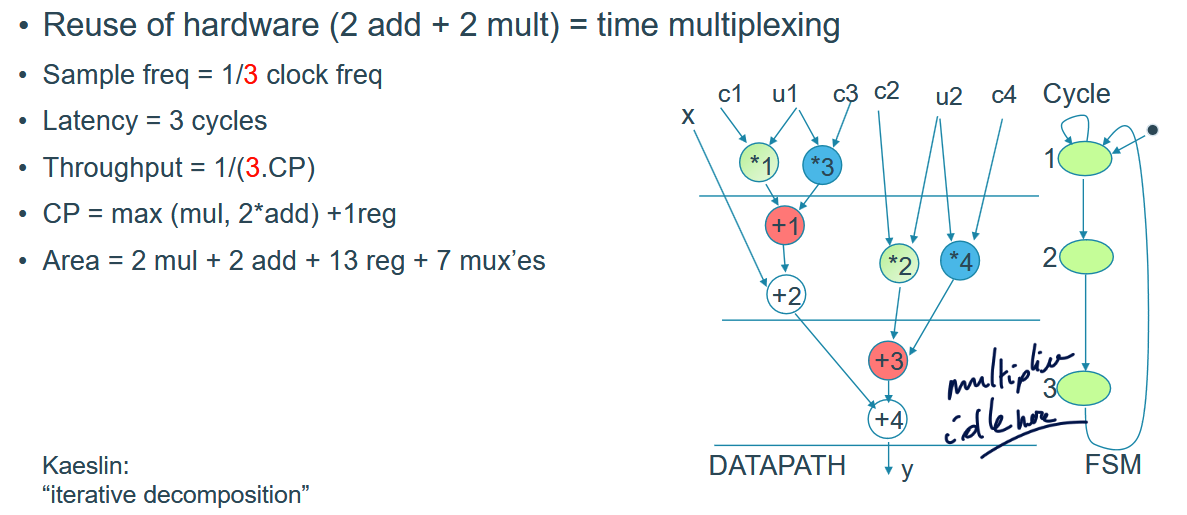
\includegraphics[width=0.45\linewidth]{img/iterative_decomposition.png}
    \caption{Slowing down : multiple datastream or reuse the same hardware}
    \label{fig:enter-label}
\end{figure}

Also something we can do is add a bit of pipelining to have a better hardware utilization, this can be done easily if we do some loop unrolling and we check at each step how we could use more of the hardware without modifying the algorithm.


\chapter{Second Part}

This is the part of Wim Dehaene which covers the physical gap triangle and works its way to the top.

\section{Throughput}

We have many strategies to have a bigger throughput. The worst throughput is through CPU since they run in \textbf{sequential} mode and so can only produce data one by one after X cycles. We can use some tricks of \textbf{pipelining, parallelism} to have more area usage but more throughput. On the other hand \textbf{time multiplexing} will have the opposite effect. We have 5 main concerns in DDP : 

\begin{enumerate}
    \item Throughput : measured in amount of data produce per cycle
    \item Latency/delay : measured in time
    \item Energy (or power) : measured in Joule or Watts
    \item Flexibility  : hard to quantify :((
    \item Area : measured in amount of LUTs, REGs, ...
\end{enumerate}

A basic relation with throughput is : 

\begin{equation}
    Throughput = \frac{1}{T_{crit. path}}
\end{equation}

The critical path has delay coming from : 
\begin{enumerate}
    \item $T_{logic}$ : due to imperfection and propagation
    \begin{itemize}
        \item $t_{pd}$ : logic propagation delay : responsible for the maximum limit
        \item $t_{cd}$ : logic contamination delay : is the minimal delay in logic
    \end{itemize}
    \item $T_{ff}$ : due to the flipflop, added overhead.
\end{enumerate}

\subsection{Sequential, synchronous design}

\subsubsection{Sequential}

The current output depends on actual and previous inputs (\textit{tokens}). It uses FSM and pipelines. We use FF and latches to remember pervious values.

\subsubsection{Synchronous}

All operation and state transition are only allowed at a specific moment that we can \textbf{clock}. All inputs must be synchronous to the same clock.

So computing is easier and we are working with stable inputs, we can clearly know when a result is valid ! It makes everything more manageable. It is \textit{deterministic} and allows us to make abstraction of the physical details.

But we are always drawn back by the critical path or the worst case delay. We have big Power consumption at each clock signal since all at once everything is running. If we want to interconnect clock domain it is hard.

The only \textbf{asynchronous signal} are \textit{reset, IO's}. So the idea is to be \textit{locally synchronous, globally asynchronous}. We need everything besides \textit{clock dividers} to have a reset signal to bring everything to a known state. Why ?

\begin{itemize}
    \item To make sure everything resets no matter how long the pulse of RST was
    \item Avoid extra delay
\end{itemize}

\subsubsection{Clock domain}

Each \textit{system} of synchronous domain are working with the same clock. But it is possible to connect multiple systems with each having their own clock domain together.

\subsection{Latch and FF}

\begin{itemize}
    \item Latch : stores data when clock is low, transparent when high (positive latch)
    \item D-FF : stores the data when clock rises
\end{itemize}

In all of this, there will some setup and hold time to make sure everything behaves as expected:

\begin{figure}[H]
    \centering
    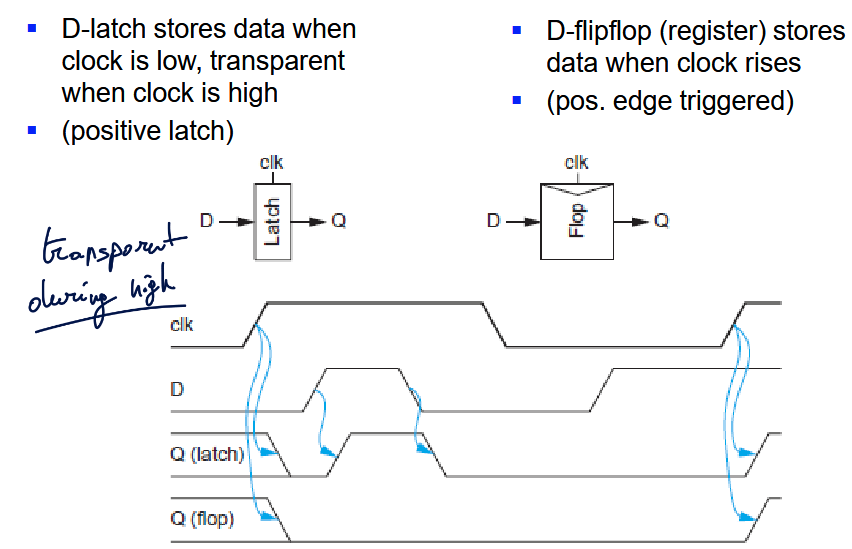
\includegraphics[width=0.75\linewidth]{img/latch_FF.png}
    \label{fig:enter-label}
\end{figure}

\begin{itemize}
    \item $t_{pcq}$ : Worst case propagation delay (so with the logic)
    \item $t_{ccq}$ : Contamination delay (min propagation delay)
    \item $t_{setup}$ : setup time, data must be valid before clock edge
    \item $t_{hold}$ : hold time, data must be valid after clock edge
\end{itemize}

But for \textbf{latches} we need to take into account :

\begin{itemize}
    \item $t_{pdq}$ : worst case propagation delay D to Q
    \item $t_{cdq}$ : contamination delay : minimum propagation delay D to Q
\end{itemize}

Because a latch is like a MUX, routed on itself ! $Q = \overline{CLK} \cdot Q + CLK \cdot D$. The setup time needs to be $t_{setup} = 3 t_{pdf\_inv} + t_{pd\_x}$. For the hold time it is $t_{hold} = t_{pd\_invc} - t_{pd\_inv1}$.

\begin{figure}[H]
    \centering
    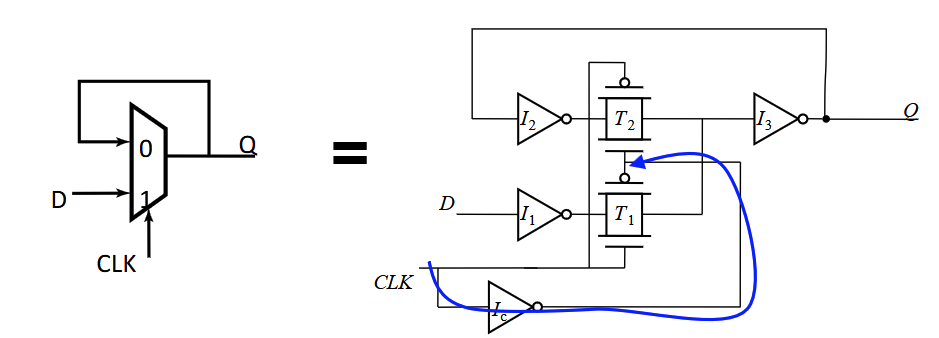
\includegraphics[width=0.7\linewidth]{img/latch.png}
    \label{fig:enter-label}
\end{figure}

\subsubsection{Metastable}

One issue that can appears is \textbf{metastability}. This can be due to a changing input that isn't properly set and so will create for a certain duration a metastability that will often get stable due to noise or other imperfection.

\begin{figure}[H]
    \centering
    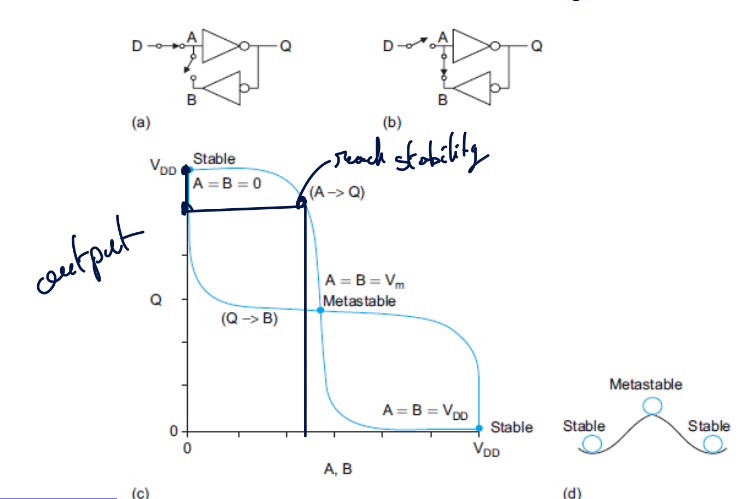
\includegraphics[width=0.75\linewidth]{img/metastable.png}
    \label{fig:enter-label}
\end{figure}

We use a model with a feedback with gain $G$ and with some resistance and capacitance. Which gives us the diff equation :

\begin{align*}
    \frac{G a(t) - a(t)}{R} &= C \frac{da}{dt}\\
    a(t) &= a(0) e^{\frac{t}{\tau}} \qquad \tau = \frac{RC}{G-1}\\
    t_{meta} &= \tau \left[ ln(\Delta V) = ln(a(0)) \right]
\end{align*}

\begin{figure}[H]
    \centering
    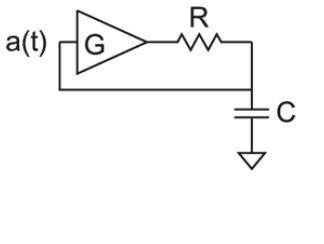
\includegraphics[width=0.3\linewidth]{img/model_meta.png}
    \label{fig:enter-label}
\end{figure}

So it is forever stable if $a(0) = 0$ but it is not feasible since there will always be some noise. With the second equation we can see that by having high gains we reduce the meta stability time.

\subsubsection{FF}

In practice, a ff is just 2 back-to-back latches. It works by using a master-slave architecture. So it creates a setup time of $t_{setup} = 3 t_{pd\_inv} + t_{pd\_x}$. And the hold time is $t_{hold} = t_{pd\_invc} - t_{pd\_inv1}$. For this implementation of the FF we have a propagation delay of $t_{cq} = t_{pd\_inv}+t_{pd\_tx}$.

\begin{figure}[H]
    \centering
    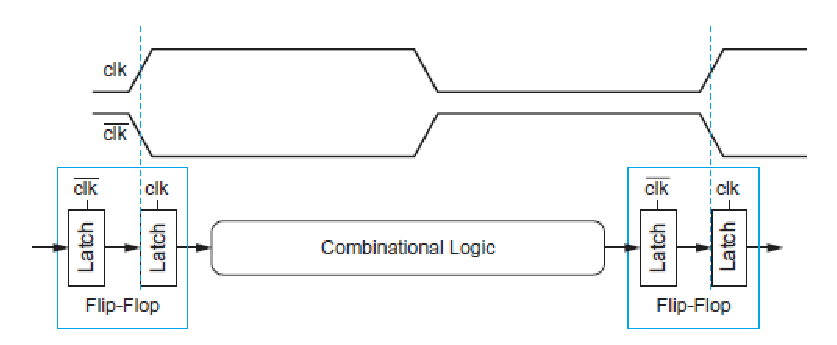
\includegraphics[width=0.75\linewidth]{img/B2B_FF.png}
    \label{fig:enter-label}
\end{figure}

\begin{figure}[H]
    \centering
    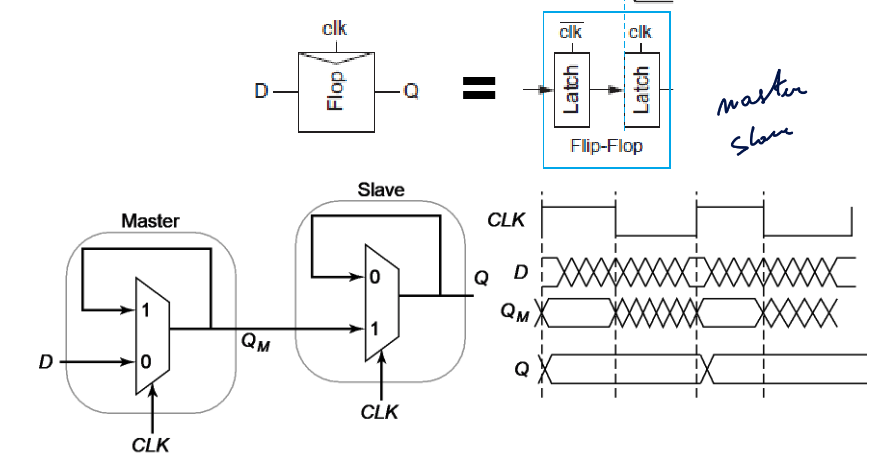
\includegraphics[width=0.75\linewidth]{img/master_slave.png}
    \caption{Master Slave configuration}
    \label{fig:enter-label}
\end{figure}

\subsection{Synchronization (I/O)}

\subsubsection{Synchronization needs}

Not all inputs are synchronized with the clock (user input, not time reference in network inputs, change of phase, mismatch, ...). This will cause some metastability issues ! So we need to add a synchronizer to make sure those asynchronous inputs cause any metastability. But those synchronizers are just flip flops !

\subsubsection{Metastability}

But as we saw previously, the metastability is pretty unstable and will lead to one of the two state either high or low. Less setup time is better and longer waiting is also better. So to synchronize we can just chain FF and just hope this stochastic process will not fail.

\subsubsection{Synchronization Mechanisms}

It would be naive to think that it is easy to synchronize registers. Even in the same registers, different data lines don't have the same delay and even worse for physically different FF.

To solve this we use \textbf{FIFO's and Handshaking}. Handshaking is like in network, we use ACK bits to communicate data between different systems. The simplest only use one handshaking lines but we can think of smarter and more resilient systems. 

\begin{figure}[H]
    \centering
    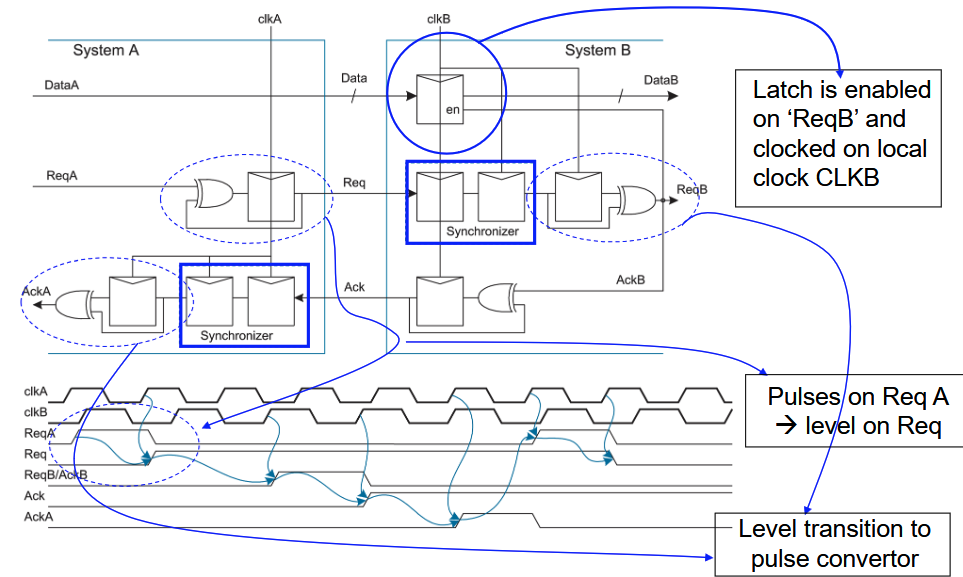
\includegraphics[width=0.75\linewidth]{img/slide_49.png}
    \label{fig:enter-label}
\end{figure}

When we use FIFO register, we write in one clock domain and read from the other. We also use some full and empty signals to indicate when the queue is full or not. 

So we need to synchronize all data that enters from another clock domain. Handshaking is required when we send more than 1 bit (to make sure the stream of bits is correctly interpreted). To build a synchronizer FF we need at least 2 FF to get rid of the metastability so it adds some delay too.

\subsection{Pipelining with real FF}

Why pipelining ? Because when we have a set of operation, each part of this set of operation is only useful for a brief moment and the data has to go through many many operators before outputing something valid which make timing constraints tougher. By pipeling (i.e. adding some registers between the operation) we are making the timing constraints easier.

\begin{itemize}
    \item + Better throughput since smaller critical path
    \item + More efficient hardware usage 
    \item - More cycles so more latency not suitable for realtime
    \item - Not so interesting when we use real flipflops since it requires a lot of energy
\end{itemize}

Latency can also be a problem for feedback loop which will decrease the throughput. Also when we pipeline, we may try to predict or start operations that will not be useful or incorrect due to feedback (X86 4 cycles fetch decode execute store issues).

\subsubsection{Setup and Hold time}

When pipeling it is important to keep this equation correct.

\begin{equation}
    T_c > t_{pd} + \underbrace{t_{pcq} + t_{setup}}_{\text{sequencing overhead}}
\end{equation}


\subsubsection{Skew and Jitter}

Skew is the fact that all clock signals won't be fired at the same time due to difference between the routing, the load etc so we talk about clock skew and is deterministic difference. Clock jitter is a statistical difference and is usualy seen as the worst case of $N \sigma $ skew. We need some good PLL to avoid any jitter. This class will focus more about skew. To avoid any setup violation

\begin{align}
    t_{pd} &\leqslant T_c - (t_{pcq} + t_{setup} + t_{skew}) & t_{cd} &\geqslant t_{hold} - t_{ccq} + t_{skew}
\end{align}

Cause of the skew, we could have the issues where some data may just pass through the register without being clocked and move on. Often in shift register since we clock on itself and execute a bit shift.

The sequencing overhead puts a limit to the amount of pipelining we can do. Skew has 2 effects

\begin{enumerate}
    \item Decreases available useful time, adds up to sequencing overhead (more setup time)
    \item Worsens hold time problem
\end{enumerate}

\section{Delay and Latency}

We want to measure and quantify the values of $t_{pd},t_{cd}$ where we mostly need to do back-of-the-envelope estimation. For $t_{pcq},t_{setup}$ we also need to do the same.

\subsection{INV}

\subsubsection{RC gate delay model}

We characterize an inverter as a circuit in two possible state, either a swithc open and a R to ground or vice versa if we have a negative input. In both cases, we need to add a load capacitance $C_L$ which creates a time constant for both of $\tau = RC$.

\begin{figure}[H]
    \centering
    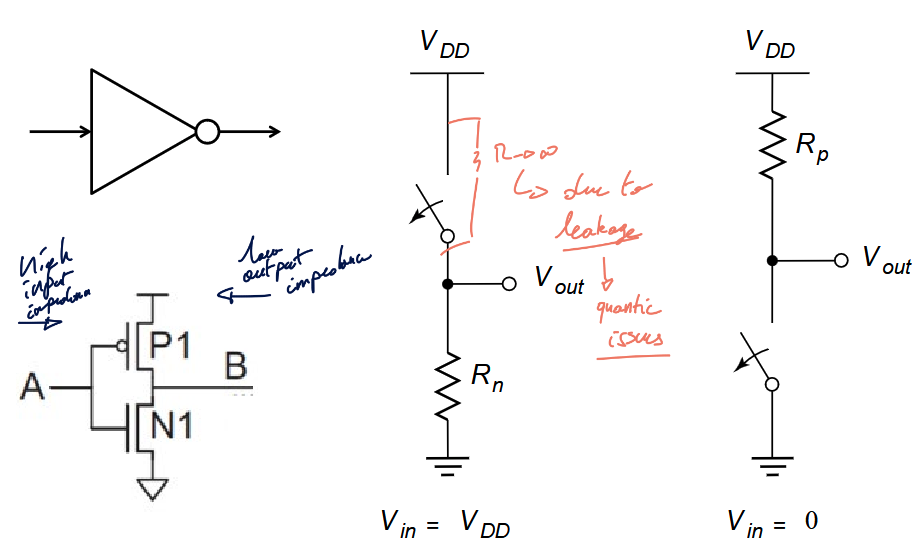
\includegraphics[width=0.75\linewidth]{img/RC_model_INV.png}
    \label{fig:enter-label}
\end{figure}

\begin{align}
    I &= C_L \frac{dV_{out}}{dt} & I &= -\frac{V_{out}}{R}\\
    V_{out}(t) &= V_{DD} e^{-t / \tau} & t_{pd} &= RC_L ln(2) 
\end{align}

This $ln(2)$ is really important for us because it indicates the exact moment in time where $V_{out}/V_{DD} = 0.5$. 

We need to make the difference between intrinsic load and extrinsic load. Intrinsic is linked with the Device Under Test. Here, we can simplify a NMOS transistor as a simple switch with a R to its drain and capacitance to all of its nodes. For a PMOS, to be more accurate we are using 2R to represent holes mobility. We can size all of transistors by a factor $k$ where it will do $kC$ and $R/k$.

When we analyze the network, we will only take into account the \textbf{Switching capacitance} since they are the one where the load will change. So here, we see that we have a $t_{pd} = 6RC ln(2) \approx 4RC$. So we can see that the transition delay $t_{pd}$ is proportional to the Resistance and capacitance. So to make a gate faster we need to make its capacitance and resistance smaller which can be done simultaneously with scaling.

From now on, we will refer the classic INV gate as the standard \textbf{delay of size 1} without load $\approx 2RC$ and with an INV load $\approx 4RC$. The reference for the cap is $C_{in\_inv} = 3C$.

\subsubsection{Linear gate delay model}

We need to distinguish the \textit{intrinsic delay} $p$ and the \textit{extrinsic delay} $f$ or effort delay.

\begin{align}
    t_p &= ln(2) \cdot R(C_{int} + C_{ext})\\
    &= \underbrace{ln(2) \cdot R_{inv1} C_{in\_inv1}}_{t_{p0}} \left( \underbrace{\frac{C_{int} R}{C_{in\_inv1} R_{inv1}}}_{p} +  \underbrace{\frac{C_{ext} R}{C_{in\_inv1} R_{inv1}}}_{f}\right)\\
    t_p &= t_{p0} d\\
    &= t_{p0} (p+f)
\end{align}

The delay is independent of the sizing since resistance go down with the size but capacitance goes up.

For the effort delay, it is dependant to the next stages that it needs to drive. It is dependant of :

\begin{itemize}
    \item The fanout of the gate $C_{ext}$
    \item The size of the gate $C_{in}$ and $R$
\end{itemize}

\begin{align}
    f&= \frac{C_{ext} R}{C_{in\_inv1} R_{inv1}} = \frac{C_{ext}}{C_{in\_inv1}S} = \frac{C_{ext}}{C_{in}}\\
    INV : t_p &= t_{p0}\left( 1 + \frac{C_{ext}}{C_{in}} \right)
\end{align}

\begin{figure}[H]
    \centering
    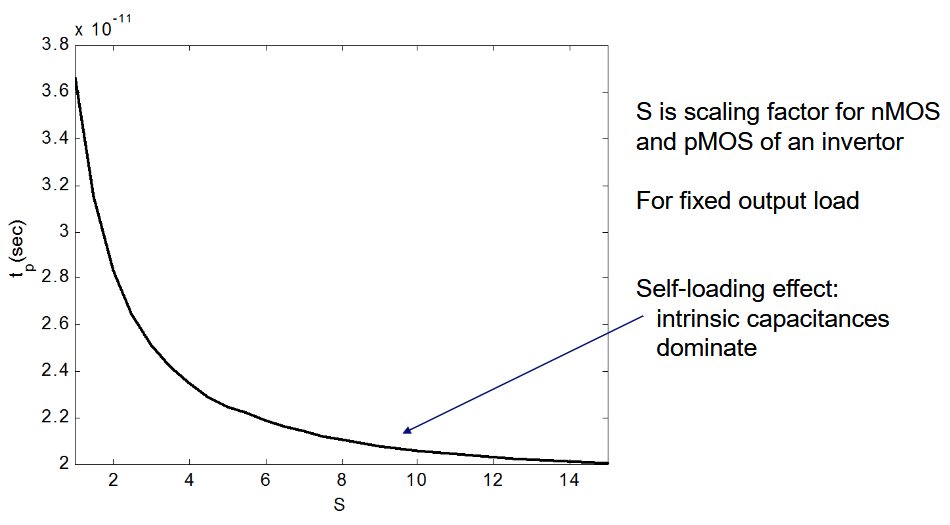
\includegraphics[width=0.5\linewidth]{img/scaling_figure.png}
    \label{fig:enter-label}
\end{figure}

If we have a fanout of 3 INV, we will have $f = 3$ and $p=1$ if we keep normal size transistor.

\subsubsection{Inverter chain optimizations at circuit level}

When we chain inverter gates which may have different size, we can simplify our RC model by having this :

\begin{align}
    t &= t_{p0}\left( 1 + \frac{C_{in2}}{C_{in1}} + 1 + \frac{C_{in3}}{C_{in2}} + ... + 1 + \frac{C_{L}}{C_{inN}} \right)
\end{align}

And thus, we can also minimize the delay by carefully picking our sizing : 

\begin{equation}
    min\left( \frac{S_{2}}{S_{1}} + \frac{S_{3}}{S_{2}} + ... + \frac{F}{S_{N}} \right) \qquad F = \frac{C_L}{C_{in,inv1}}
\end{equation}

To minimize this delay we must have : 

\begin{equation}
    S_j = \sqrt{S_{j-1}S_{j+1}}
\end{equation}

This make sure every stages have the same effort $f$ and so have the same delay ! $t_{p0}(1+f)$

If we know the input and load capacitance we can also do the same procedure to find the optimal sizing where $F = f^N$ and $N = log_f F = \frac{ln(F)}{ln(f)}$. Which gives us:

\begin{align}
    t_p &= Nt_{p0}(1+f) = t_{p0} ln(F)\left( \frac{f}{ln(f)} + \frac{1}{ln(f)} \right)\\
    \frac{\partial t_p}{\partial f} &= t_{p0} ln(F) \frac{ln(f) - 1 - \frac{1}{f}}{ln^2(f)} = 0\\
    f &= exp(1 + 1/f) \quad f_{opt} \approx 3.6
\end{align}

Since we found the optimal effort, we can find an optimal amount of stage that will satisfy as close as possible the speed. 

\begin{equation}
    f_{opt}^{N_{opt}} = F \quad N_{opt} = \frac{ln(F)}{ln(f_{opt})} \quad t_p = Nt_{p0} (1+\sqrt[N]{F})
\end{equation}

If we deviate from the actual number of stages it is not that sensitive so it's okay to go one more or one less. But mis-sizing is a bit more impactful.

\subsection{Other Gates}

We can simplify all of the other gates as a Pull-Up network and a Pull-Down network. The easiest thing to do for designing is having an inverted logic expression and then start with the pull down. After this we can to the same for the pull up and inverse everything. The PUN needs to be of size $2$ and PDN of size $1$. In series we do $1/(1/S_1+1/S_2)$ and in parallel $(S_1+S_2)/2$

\subsubsection{Linear gate delay model}

We can reuse the linear gate model but this time with a twist : 

\begin{align}
    t_p &= ln(2) \cdot R(C_{int} + C_{ext})\\
    &= \underbrace{ln(2) \cdot R_{inv1} C_{in\_inv1}}_{t_{p0}} \left( \underbrace{\frac{C_{int} R}{C_{in\_inv1} R_{inv1}}}_{p} +  \underbrace{\frac{C_{ext} R}{C_{in\_inv1} R_{inv1}}}_{f=g.h}\right)
\end{align}

Where $g$ is the \textbf{logical effort} due to the sizing difference with an INV and $h$ is the \textbf{electrical effort} ($C_{out}/C_{in}$).

The \textit{parasitic delay} $p$ of a gate is the delay of the gate when it drives zero load normalized to an inverter that drives equal current (same R). To find $C_{int\_S1}$ we just look at the output node and the amount of capacitance connected to it.

\begin{equation}
    p = \frac{C_{int\_S1}}{C_{in\_inv\_S1}} =  \frac{C_{int\_S1}}{3}
\end{equation}

The \textit{logical effort} $g$ of a gate is the ratio of its \textit{input capacitance} to that of an inverter that has equal R. This value doesn't scale up over the sizing.

\begin{equation}
    g =  \frac{C_{in\_S1}}{C_{in\_inv\_S1}}
\end{equation}

The \textit{electrical effort} $h$ is simply $C_{ext}/C_{in}$ where we can express all of the capacitance as the normal size $C_{in,inv}$ times a certain factor $g$. Example, with a 3 NAND followed with a NOR we see that $C_{in} = g_{nand3}C_{in,inv}$ and $C_{ext} = g_{or} C_{in,inv}$. $h = g_{or} / g_{nand3}$. If we size the NAND and NOR by a and b then $h = b g_{xor} / a g_{nand3}$ :

\begin{align}
    C_{in} &= size\_current \cdot g\_current & C_{ext} &= size\_next \cdot g\_next
\end{align}

\subsubsection{Multi-gate chain optimizations at circuit level}

To have the optimal delay, we need that each stages do the \textbf{same effort} not the same delay !

\begin{equation}
    g_1h_1 = g_2h_2 = ... = g_Nh_N = f
\end{equation}

The effective fanout of each stage is $h_i = f/g_i$ to have the same extrinsic delay per stage. so. 

\begin{figure}[H]
    \centering
    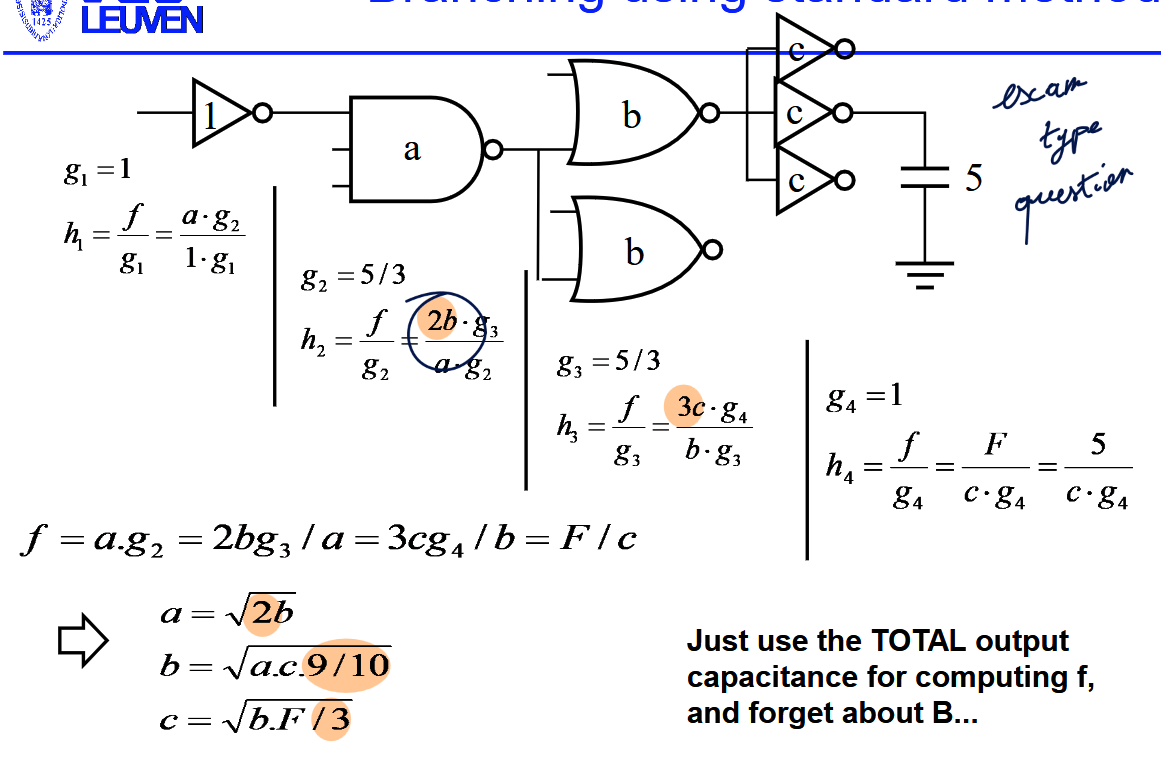
\includegraphics[width=0.75\linewidth]{img/branching.png}
    \label{fig:enter-label}
\end{figure}

\section{Power and Energy Consumption}

\subsection{Power and Energy}

\begin{itemize}
    \item We need to remember that power is an amount of energy of a time duration and it determines that battery life in hours $Watts$. 
    \item Energy efficiency is in $Joules$ and so we can find $E = P \cdot t$. So a lower energy number means less power to perform a computation at the same frequency (otherwise not comparable).
\end{itemize}

So we can have high peak power at fraction of the time and it won't use too many energy.

\subsection{Designing for Energy}

\subsubsection{Dynamic energy}

It is the power needed to flip the gates, to charge and discharge the capacitance load.

\begin{equation}
    P = fE = \alpha f CV_{DD}^2
\end{equation}

We have the $\alpha$ or \textbf{activity factor}. We need to keep in mind $C$ is not the same for all possible states, we need to count only the one that switches. We also need to remember that this formula is calculating the energy needed to \textbf{charge or discharge} not the energy stored ! The energy stored in a cap is $CV_{DD}^2 / 2$ but the source needs to provide  $CV_{DD}^2$ for it to charge it !

\begin{figure}[H]
    \centering
    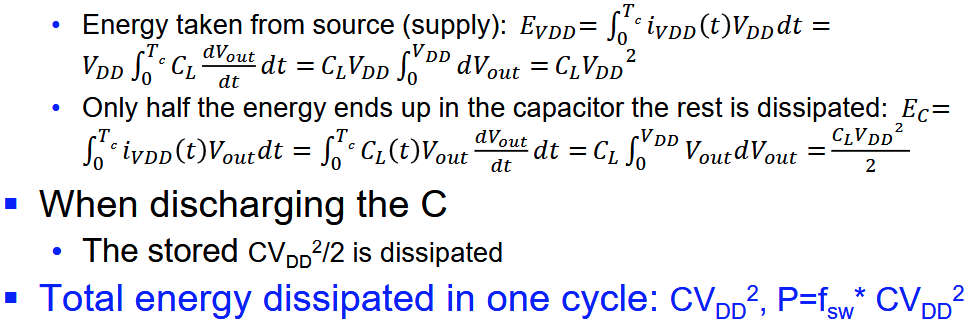
\includegraphics[width=0.75\linewidth]{img/chargecap.png}
    \label{fig:enter-label}
\end{figure}

For a simple INV + load cap, we have $E_{inv1} \approx V_{dd}^2C_{eff}$ with $C_{eff} = C_{int} + C_{in\_load} = C_{in}(f+F)$ with $f$ being the sizing factor. It is also important to take into account the cap of the wire.

\begin{figure}[H]
    \centering
    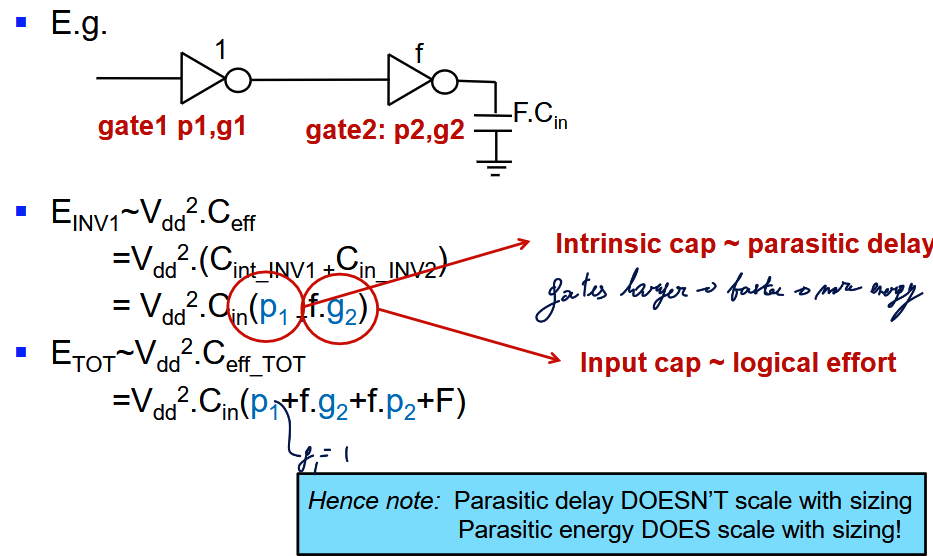
\includegraphics[width=0.65\linewidth]{img/chain_energy_2.png}
    \label{fig:enter-label}
\end{figure}

The minimal delay is not the most energy efficient. We can find trade-off between the delay $D_{min}$ and the energy. We know the energy is proportional to the $f$, so we can choose what is the best for us. Some important FOM are :

\begin{itemize}
    \item \textbf{PDP} : power-delay product : $P_{av} \cdot t_p$ which is the energy it takes to switch in time $t_p$.
    \item \textbf{EDP} : energy-delay product : $PDP \cdot t_p$ energy for delay. It shows the energy for performance. It is a really interesting FOM for embedded systems and low energy design. 
\end{itemize}

\begin{figure}[H]
    \centering
    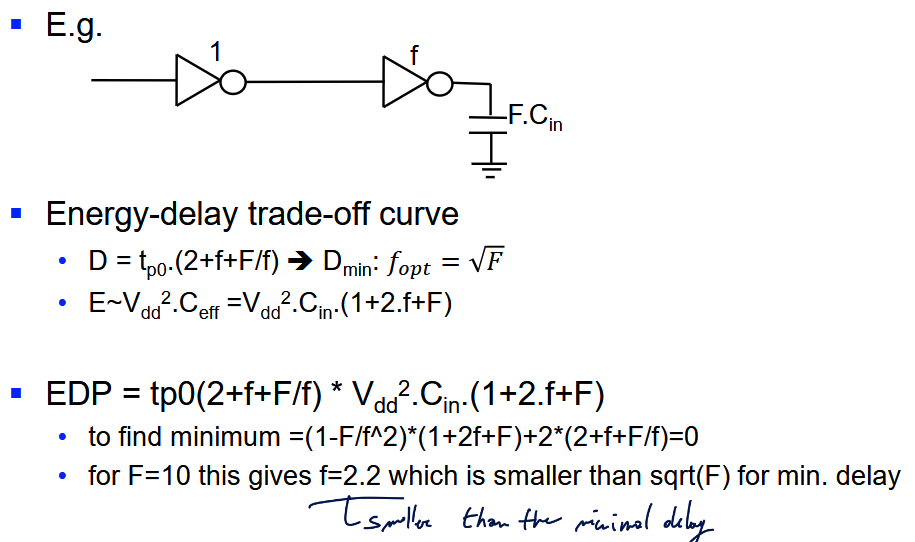
\includegraphics[width=0.75\linewidth]{img/min_edp.png}
    \label{fig:enter-label}
\end{figure}

$V_{dd}$ can be also scaled down to reduce the energy. So the energy goes down by a factor $V_{DD}^2$. But this also impact the speed since we need to charge a capacitance and we are working with transistor in saturation so $I ~ (V_{DD}-V_{th})^\alpha$. Following \textit{Sakurai's} model we can say that for long channel $\alpha = 2$ and for short we have $\alpha \approx 1.3$. So the delay is around $V_{DD}/(V_{DD} - V_{th})^{\alpha}$.

\begin{figure}[H]
    \centering
    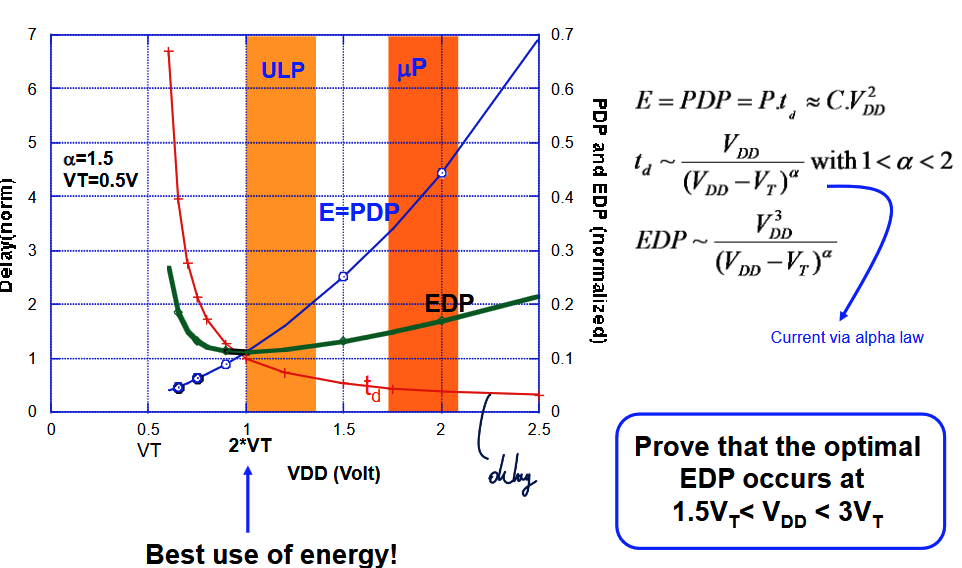
\includegraphics[width=0.75\linewidth]{img/VDD_scaling.png}
    \label{fig:enter-label}
\end{figure}

So we can do both Voltage and size scaling which allow us to go even smaller.

We can also modify the architecture to have a better impact. We can use some pipelining, etc.

\begin{figure}[H]
    \centering
    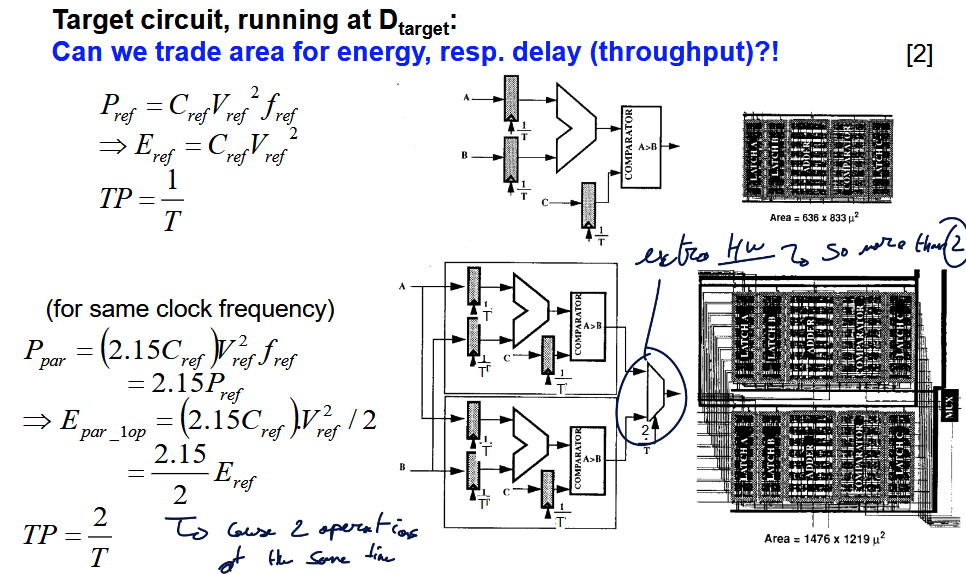
\includegraphics[width=0.75\linewidth]{img/parallelism.png}
    \label{fig:enter-label}
\end{figure}

\begin{itemize}
    \item Parallelize : we can add more hardware to parallelize operation and by having a higher throughput. But this will consume more energy so we need to slow down the operation by using a smaller $V_{DD}$ which will add more delay. But seeing how things scale with the voltage, we will use less energy for the same throughput.
    \item Pipe : we add some registers, if we keep the same $V_{DD}$ it won't help since we will flip for transistors and so higher power usage. But if we reduce this voltage to make it slower because adding a register relax timing constraint, we can make some block behaves a bit slower.
\end{itemize}

\begin{figure}[H]
    \centering
    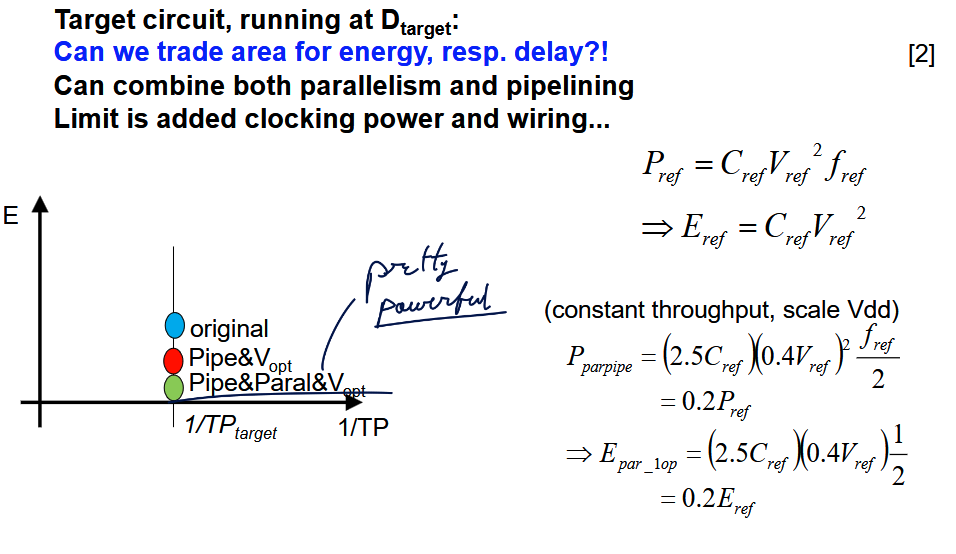
\includegraphics[width=0.75\linewidth]{img/pipe_par.png}
    \caption{There is no free lunch since we have higher area usage}
    \label{fig:enter-label}
\end{figure}

We can't reduce the $V_{DD}$ forever because leakage will become predominant. Moreover, the more hardware the bigger is the leakage current on the overall board and so one strategy is to disable portion of hardware but it is not really feasible. So dynamic energy and leakage comes into \textbf{contradiction}.

\subsubsection{Static energy}

\begin{equation}
    I_{leak} = I_0 e^{\frac{-V_T}{nkT/q}}
\end{equation}

It is associated with the leakage and so is a form of stochastic process that we average out to the mean value of this \textbf{leakage current}. But the $V_{dd}$ is exponentially dependent on the $- V_T$ so we need to be careful.

\begin{align}
    P_{stat} &= V_{dd} \cdot I_{leak} & E_{stat} &= V_{dd} \cdot I_{leak} \cdot t_d\\
    I_{leak} &= \cdot 12 \text{ per 100 mV } V_T \text{ decrease} & I_{leak} &= \cdot 2 \text{ per } 10^\circ \text{ C}
\end{align}

\begin{figure}[H]
    \centering
    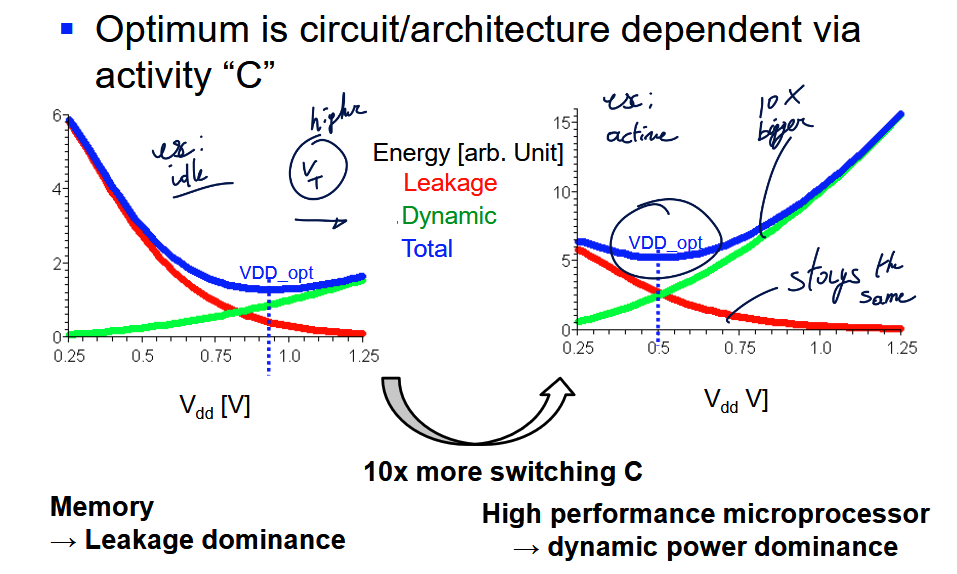
\includegraphics[width=0.75\linewidth]{img/dynamic_power_static.png}
    \label{fig:enter-label}
\end{figure}

\subsection{Low-power run-time techniques}

We will always try to get rid of \textit{unnecessary} activity, reduce supply voltage or run the clock slower. But we can do this up to a certain extent.

\subsubsection{(Dynamic) Voltage Scaling}

The optimal $V_{DD}$ is \textbf{dynamic} and depend on the minimum point of energy according to the energy per cycle targeted, how much leakage we allow, ... We can change the frequency with a \textit{VCO} but this only helps the power not the energy. A \textbf{DVFS} saves both since it touches at the $V_{DD}$.

\begin{figure}[H]
    \centering
    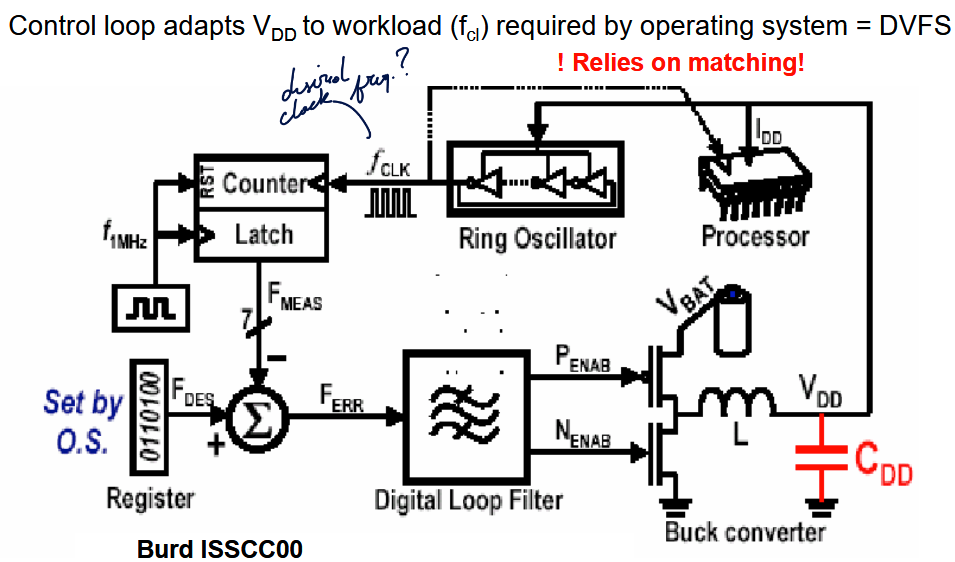
\includegraphics[width=0.75\linewidth]{img/DVFS.png}
    \caption{A rather old version of a DVFS}
    \label{fig:enter-label}
\end{figure}

This really helps by wasting less energy and often we use a power supply with a set of distinct voltages rather than something continuous because it is too expensive.

\subsubsection{Signal and Clock gating}

We try to reduce the activity of the flipping $\alpha$ by stopping the propagation of the signal to unnecessary logic. But again, we may need more circuitry and so more power. We need to have a control signal that has a frequency that is \textbf{much lower} than the source signal (like don't switch all the time the control logic or it's stupid). Try to share this control signal across multiple block. We can reuse some control signal like BUS, clock, ACK, ...

We can gate input signal from a block by using a latch that is either on or off and so propagate to another block.

\begin{figure}[H]
    \centering
    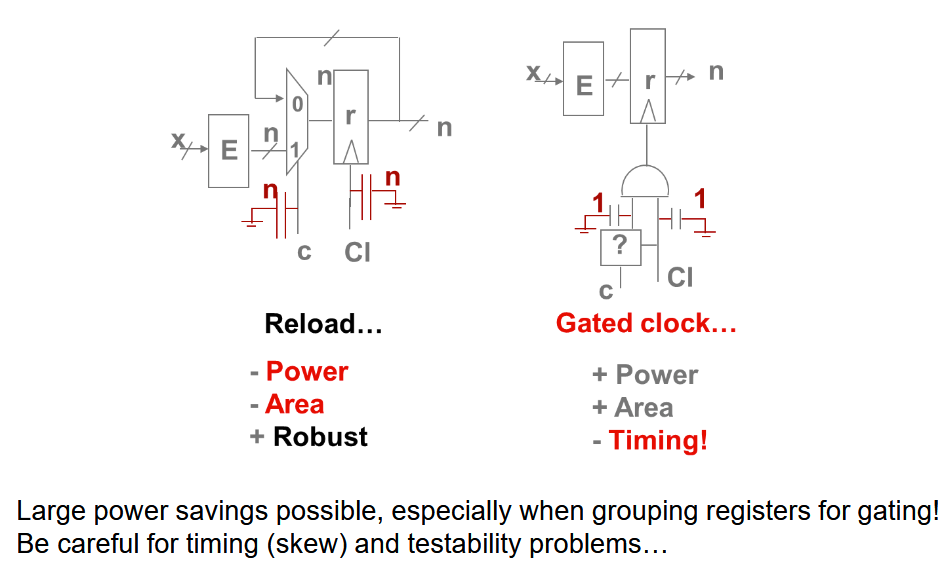
\includegraphics[width=0.75\linewidth]{img/gate.png}
    \label{fig:enter-label}
\end{figure}

\subsubsection{Power gating \& System level power management}

We know that the higher the leakage, the higher is the minimum energy point. So this is annoying for memory for example and we need to recharge the nodes all the time almost. We will try to put some part of the circuit into hibernating state but we may loose some states and time to wake up the circuit.

\begin{figure}[H]
    \centering
    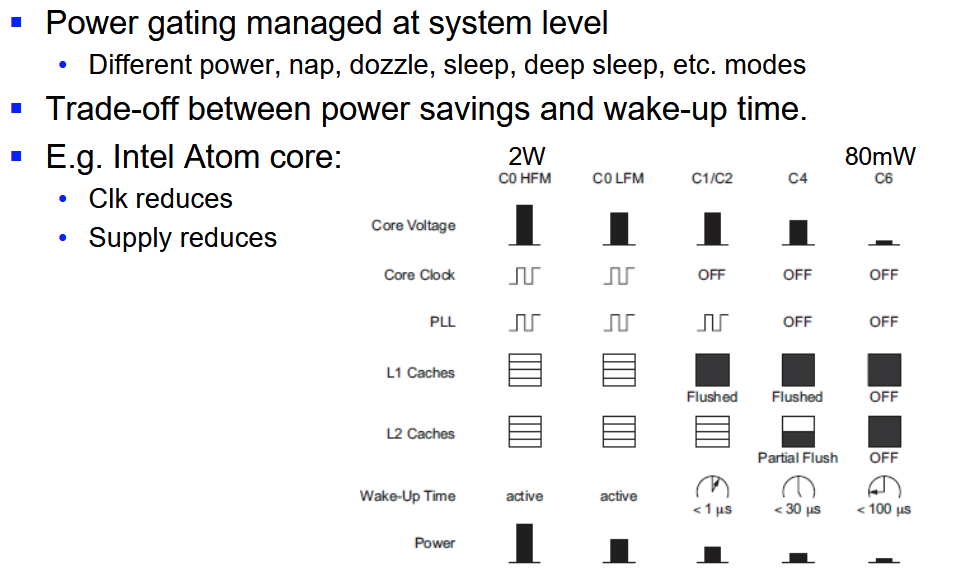
\includegraphics[width=0.5\linewidth]{img/hibernating.png}
    \caption{Hibernating}
    \label{fig:enter-label}
\end{figure}

\section{Flexibility \& Scaling}

It is hard to quantify the flexibility but often, as a platform is more dedicated and so less flexible the more efficient it is.

\subsection{What platform?}
\subsubsection{Control flow mapping: from FSM to processor}
Control flow graph can be messy and complex due to conditional loop, resource sharing, exception handling,... Which can make hardware development much much harder ! So sometimes it is better to have a more flexible hardware and control it through software which helps debugging and adapting the hardware on the go. So instead of using a FSM where we check conditions and do some logic to determine next stage, we let the software indicate what state it is now through a command register. 

By using command register and building a specific CSR, we can use the hardware with an encoder / decoder that will decrypt the CSR and translates it to actual control signal on the board. But, this will induce more muxes so bigger critical path, ... This idea is the birth of instructions sets and modern X86, ARM, RISC-V, ... It is more flexible but less efficient than ASIC.

\begin{figure}[H]
    \centering
    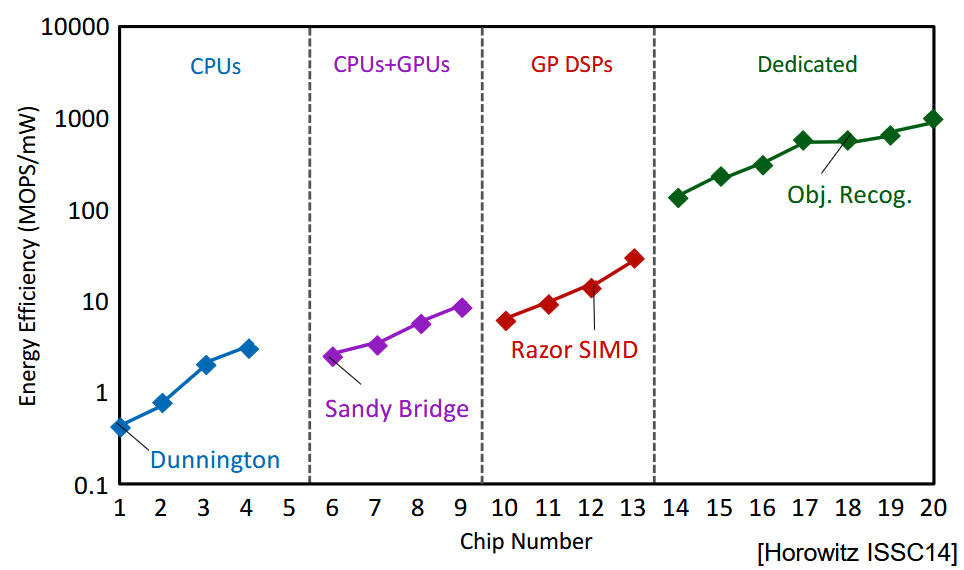
\includegraphics[width=0.75\linewidth]{img/efficiency.png}
    \label{fig:enter-label}
\end{figure}


\subsubsection{Heterogeneous HW/SW systems-on-chip}

In dataflow, we can have : 

\begin{itemize}
    \item Regular, loop intensive, high throughput:
    \begin{itemize}
        \item Dedicated Data Paths (co-processors)
        \item  SIMD arrays (= parallel datapath: single instruction, multiple data)
    \end{itemize}
    \item Irregular, low throughput, complex, programmable:
    \begin{itemize}
        \item DSP (digital signal processor),
        \item ASIP (application specific integrated processor)
    \end{itemize}
\end{itemize}

Control flow can be low power, low area or high performance with FSMD synthesis but not flexible or low performance but using flexible algorithms so micro-controller (MCU). Often, the best decision is to balance this and have a co-design approach to design some small SOC that will run specific algorithms.

The most simple way to communicate between HW and SW is using the memory BUS but this can lead to bottle neck quickly and synchronization issues if they come from 2 different clock domain. To synchronize we can either use a mailbox approach with req, ack (like in Erlang).

We can transfer $v$ bits after $B$ cycles for a transfer and we can have a result of $w$ bits every $H$ cycles. 

\begin{itemize}
    \item Computation constraint : $\frac{v}{B} > \frac{w}{H}$
    \item Communication constraint : $\frac{v}{B} \leqslant \frac{w}{H}$
\end{itemize}

If we are limited cause of the on-chip BUS we can also have a dedicated data transfer line between the software and hardware. It makes things a bit more complicated but we can send more data and go much faster (less RC). One of the best way is by using some FIFO queues with some monitoring signal like \textit{exists, full}. We often send big chunks like this than in a mailbox approach it's smaller frames. But fast and big memory is energy and power hungry.

\subsection{In what silicon technology?}

First it was a free lunch, smaller = faster = less power/energy = less area = cheaper.

\subsubsection{Device scaling (“front-end”)}

Front-end is everything related to the device so the size of the transistor. Here we will refer to the geometry scaling with $1/S$ and voltage scaling with $1/U$ for quickly understanding its impact.

\begin{enumerate}
    \item \textbf{Fixed Voltage scaling} : $S>1, U=1$ : so everything is using the same $V_{DD}$ better compatibility between technology. But we will create more heat, ...
    \item \textbf{Full scaling} or Dennard Scaling: $S=U>1$ : the idea is to keep the electric field constant $V/L$. But not everything scales like $V_T$. 
    \item \textbf{General scaling} : $S>U>1$ : We can scale the voltage up until a certain point and we can't always follow $S$.
\end{enumerate}

\begin{figure}[H]
    \centering
    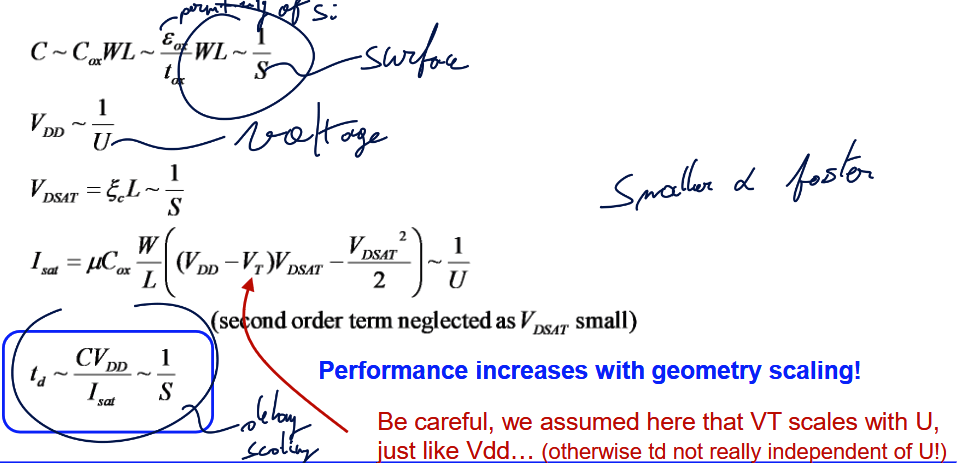
\includegraphics[width=0.75\linewidth]{img/scaling_gate.png}
    \label{fig:enter-label}
\end{figure}

\begin{figure}
    \centering
    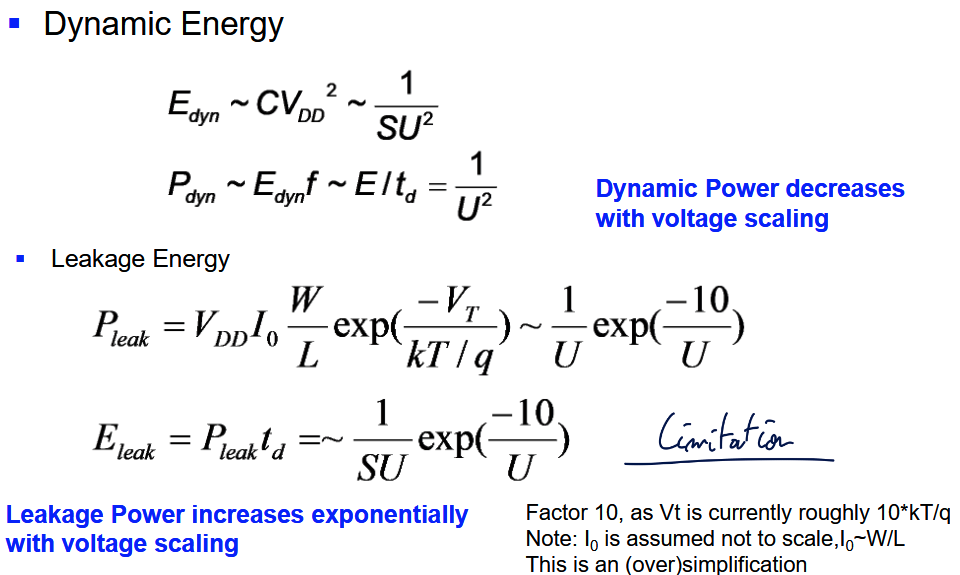
\includegraphics[width=0.75\linewidth]{img/energy_scaling.png}
    \label{fig:enter-label}
\end{figure}

\begin{table}[H]
    \centering
    \begin{tabular}{|c|c|c|c|}
        \hline
        Parameter & General Scaling $S>U>1$ & Fixed Voltage $S>1, U=1$ & Constant E field $S=U>1$\\
        \hline
$t_d$ & $1/S$ & $1/S$ & $1/S$\\
        \hline
$E_{dyn}$ & $1/SU^2$ & $1/S$ & $1/S^3$\\
        \hline
$P_{dyn}$ & $1/U^2$ & $1$ & $1/S^2$\\
        \hline
Area & $1/S^2$ & $1/S^2$ & $1/S^2$\\
        \hline
$P_{density}$ & $S^2 /U^2$ & $S^2$ & $1$\\
        \hline
    \end{tabular}
    \caption{Scenario and impact}
    \label{tab:my_label}
\end{table}

The heat increases quadratically for \textit{fixed voltage scaling} but the increase is less dramatic for \textit{general scaling}. The optimal idea is to use constant electric field scaling but not everything scales and the leakage can get too big.

\textbf{DDSM scaling}, the main drawbacks are \textit{leakage} (gets too big if VT scaling is maintained), \textit{interconnect} (wires delay is bigger than the logic) and \textit{variability} (needs to add too much buffer so we lose the gain).

\begin{figure}[H]
    \centering
    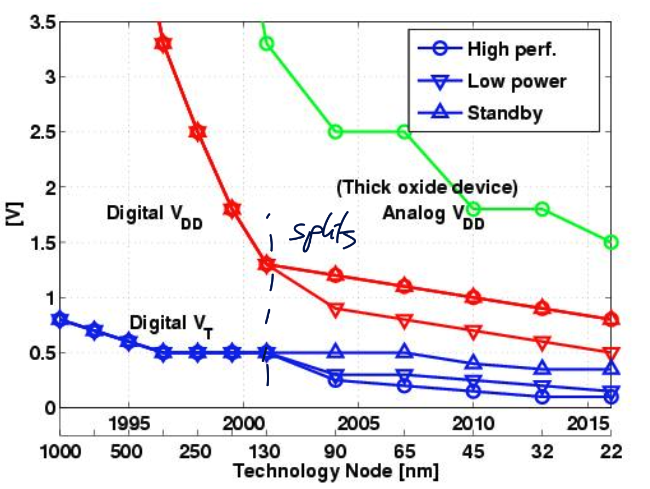
\includegraphics[width=0.75\linewidth]{img/scaling.png}
    \label{fig:enter-label}
\end{figure}

\subsubsection{Interconnect scaling (“back-end”)}

Back-end is everything related to the wiring of all the devices together so wires,... We have wires that are next to each other but also form a sort of capacitance with a potential ground plane or other wires. The timing for a wire is : 

\begin{equation}
    t_{wire} = \frac{RC}{2} = \frac{rcL^2}{2} \sim \rho \epsilon \frac{L^2}{\lambda^2} \sim \rho \epsilon L^2 S_I^2 
\end{equation}

Where $\lambda$ is the size and spacing of the wires approximately and $\lambda \sim 1/S_l $, $c\sim 1$, $r \sim 1/\lambda^2$. In general, the local connection between the gates scales down so $L \sim 1/S_l$ but since we are making more complex modules they tend to take the same amount of space so $L = cst$ for global interconnection.

\begin{align}
    T_{wire,local} &\sim L^2 S_l^2 & T_{wire,global} &\sim S_l^2
\end{align}

But the energy also varies with the sizing. Again with the same idea that local wiring scales down but not global. But the energy goes by a 3 order for local with constant electric field and quadratically for global wires.

\begin{equation}
    E_{wire} = C_{wire} V_{DD}^2 \sim \epsilon \frac{\lambda L}{\lambda} V_{DD}^2 \sim \frac{L}{U^2}
\end{equation}

\subsubsection{Variability}

By going smaller and smaller, when doping one region, $\pm$ 1 ion make a much much bigger difference in the doping ! So, $V_T$ can vary a lot and we have some \textit{inter-die} and \textit{intra-die} effects. We can use some good matching practices.

\begin{figure}[H]
    \centering
    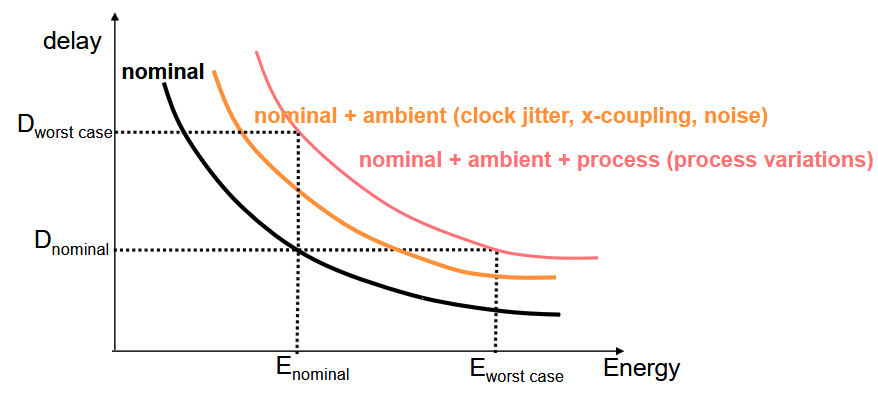
\includegraphics[width=0.75\linewidth]{img/margin.png}
    \caption{More and more margin needed}
    \label{fig:enter-label}
\end{figure}

\textbf{Systematic variations} are the same for all TORs on the die but different for different die (inter-die), we can do some delay monitoring and tuning. \textbf{Random variations} vary from one transistor to the other (intra-die), we can add some margin.

We really are aiming at low energy for more functionality. We need to deal more and more with variability and leakage, the free lunch era is over. Need of good engineers and creative one especially !

\end{document}
